%%%%%%%%%%%%%%%%%%%%%%%%%%%%%%%%%%%%%%%%%%%%%%%%%%%%%%%%%%%%%%%%%%
%%%%%%%% ICML 2016 EXAMPLE LATEX SUBMISSION FILE %%%%%%%%%%%%%%%%%
%%%%%%%%%%%%%%%%%%%%%%%%%%%%%%%%%%%%%%%%%%%%%%%%%%%%%%%%%%%%%%%%%%

% Use the following line _only_ if you're still using LaTeX 2.09.
%\documentstyle[icml2016,epsf,natbib]{article}
% If you rely on Latex2e packages, like most moden people use this:
\documentclass{article}

% use Times
\usepackage{times}
% For figures
\usepackage{graphicx} % more modern
%\usepackage{epsfig} % less modern
%\usepackage{subfigure} 

% For citations
\usepackage{natbib}

% For algorithms
\usepackage{algorithm}
\usepackage{algorithmic}
\usepackage{graphicx}
\usepackage{amsfonts}
\usepackage{amsmath}
\usepackage{amsthm}
\usepackage{booktabs}
\usepackage[percent]{overpic}
\usepackage{csquotes}
%\usepackage[lined,boxed,commentsnumbered,ruled]{algorithm2e}
\usepackage{color}
\usepackage{caption}
\usepackage{subcaption}
\usepackage{xspace}
\usepackage{verbatim}
\usepackage{multirow}

% As of 2011, we use the hyperref package to produce hyperlinks in the
% resulting PDF.  If this breaks your system, please commend out the
% following usepackage line and replace \usepackage{icml2016} with
% \usepackage[nohyperref]{icml2016} above.
%\usepackage{hyperref}

% Packages hyperref and algorithmic misbehave sometimes.  We can fix
% this with the following command.
\newcommand{\theHalgorithm}{\arabic{algorithm}}

\newcommand{\BB}[1]{\textcolor{red}{\bf Byron: {#1}}}
\newcommand{\arun}[1]{\textcolor{red}{\bf Arun: {#1}}}
\newcommand{\drew}[1]{\textcolor{blue}{\bf Drew: {#1}}}
\newcommand{\wen}[1]{\textcolor{green}{\bf Wen: {#1}}}
\newcommand{\geoff}[1]{\textcolor{green}{\bf Geoff: {#1}}}

\newcommand{\todo}{\textcolor{red}{\textbf{[TODO]}}}

\newcommand{\pbim}{\textsc{PSIM}\xspace}
\newcommand{\PBIM}{\textsc{Predictive State Inference Machine}\xspace}

\newcommand{\pbims}{\textsc{PSIM}s\xspace}
\newcommand{\PBIMs}{\textsc{Predictive State Inference Machines}\xspace}


\newtheorem{theorem}{Theorem}[section]
\newtheorem{lemma}[theorem]{Lemma}
\newtheorem{proposition}[theorem]{Proposition}
\newtheorem{corollary}[theorem]{Corollary}
\newenvironment{definition}[1][Definition]{\begin{trivlist}
\item[\hskip \labelsep {\bfseries #1}]}{\end{trivlist}}




% Employ the following version of the ``usepackage'' statement for
% submitting the draft version of the paper for review.  This will set
% the note in the first column to ``Under review.  Do not distribute.''
\usepackage{icml2016} 

% Employ this version of the ``usepackage'' statement after the paper has
% been accepted, when creating the final version.  This will set the
% note in the first column to ``Proceedings of the...''
%\usepackage[accepted]{icml2016}


% The \icmltitle you define below is probably too long as a header.
% Therefore, a short form for the running title is supplied here:
\icmltitlerunning{Deeply AggreVaTeD: \\ Imitation Learning }

\begin{document} 

\twocolumn[
%\icmltitle{Differentiable Imitation Learning and Structured Prediction}
\icmltitle{Needs better title\\ expect two lines.}


%\icmltitle{Differentiable Imitation Learning and Structured Prediction}

% It is OKAY to include author information, even for blind
% submissions: the style file will automatically remove it for you
% unless you've provided the [accepted] option to the icml2016
% package.
\icmlauthor{Wen Sun$^{\dagger}$}{wensun@cs.cmu.edu}
\icmlauthor{Arun Venkatraman$^{\dagger}$}{arunvenk@cs.cmu.edu}
\icmlauthor{Byron Boots$^*$}{bboots@cc.gatech.edu}
\icmlauthor{J. Andrew Bagnell$^{\dagger}$}{dbagnell@ri.cmu.edu}
\icmladdress{$^\dagger$Robotics Institute, Carnegie Mellon University, USA \\
$^*$College of Computing, Georgia Institute of Technology, USA 
}
%\icmladdress{$^\dagger$ Robotics Institute, Carnegie Mellon University, Pittsburgh, PA, USA}
% You may provide any keywords that you 
% find helpful for describing your paper; these are used to populate 
% the "keywords" metadata in the PDF but will not be shown in the document
\icmlkeywords{boring formatting information, machine learning, ICML}

\vskip 0.3in
]

% \begin{abstract}
% %Imitation Learning (IL) is an important tool for learning policies by imitating an expert.
% \drew{Comment above doesn't have a lot in it}
% Following previous work on imitation learning \cite{ross2014reinforcement}, we introduce \emph{Differentiable Imitation Learning} (DIL) \drew{Let's not make it a totally different name since we're basically showing the deep version of Aggrevate}, a family of policy gradient methods for IL. DIL is specifically designed to learn policies modeled by complex function approximators such as neural networks. We also provide a comprehensive theoretical study of IL on finite discrete Markov Decision Process (MDP) to show that IL, in general, can learn much faster than Reinforcement Learning (RL). We experimentally demonstrate a stochastic gradient update procedure and a natural gradient update procedure on high-dimensional continuous robotics control tasks and a partially observable dependency parsing task on raw image data. In practice, we show that DIL, with both feedforward and recurrent neural network policies, can achieve expert-level performance and often surpasses sub-optimal experts.
% \end{abstract}


\begin{abstract}
Deep learning models are advancing the state of the art in structured prediction, but increasingly require training that goes beyond traditional supervised learning regimes. \cite{} Researchers have begun adopting reinforcement learning algorithms to train such structued predictors. We argue here that \textit{AggrevaTeD}-- a policy gradient extension of the Imitation Learning approach of \cite{Ross}-- leads to faster and better solutions with less training data then relying on less-informed RL techniques.  With both feedforward and recurrent neural predictors, we demonstrate stochastic gradient procedures to solve high dimensional continuous control problems as well as a partially observed dependency parsing task from raw image data. Backing our empirical findings, we provide a comprehensive theoretical study of IL that demonstrates we can expect \textit{exponentially} lower sample complexity for learning with \textit{AggrevateD} then with Reinforcement Learning algorithms. In both practice and in theory \drew{should we carefullly note this int he appendix since this has been a point of confusion for some folks?} we observe that the approach can achieve performance beyond that of the demonstrator when the demonstrator is sub-optimal. \drew{Needs some work. bb take pass.}
\end{abstract}



%\vspace{-10pt}
\section{Introduction}
\label{sec:intro}
\BB{The paper does not discuss structured prediction much. We could either make it more prominent in the introduction and throughout, or ignore it (and remove from title) until the experimental results where we say something about how we can also use for structured prediction.} \drew{I think the paper is supposed to be saying IL > RL for structured prediction,and demonstrating the application of IL to deep networks. I think it's basically a paper teaching people how/when to use IL, particularly to train networks. How do we get it there?} 
A fundamental challenge in artificial intelligence, robotics, and controls, is to find a policy that maps state to actions to minimize accumulated cost or achieve a goal. A promising approach to this problem is Imitation Learning (IL), which automatically learns a policy from expert demonstrations.  IL has become an important tool in a range of fields including robotics \cite{Ross2011_AISTATS} \drew{Is that the right ref}, statistical inference \cite{ross2011_CVPR,sun2016learning}, and language parsing \cite{chang2015learning_dependency}. 

Classical imitation learning \cite{abbeel2004apprenticeship,syed2008apprenticeship,ziebart2008maximum,finn2016guided,ho2016generative} learns a policy from a fixed-size dataset pre-collected from experts. The learned policy intends to match the expert's behaviour in terms of either the expected feature counts of visited states (e.g., MaxEnt \cite{ziebart2008maximum}) or the entire distribution of demonstrated trajectories \cite{ho2016generative}. A pernicious problem with these classical methods is that they require the training and test data to be sampled from the same distribution.  This is very difficult to enforce in practice, and, as a result, policies learned by these methods can fail spectacularly in real-world scenarios~\cite{ross2010efficient}.

\drew{I feel we are talking a lot about IL, and not about our contribution...}

Interactive learning approaches to IL such as SEARN \cite{daume2009search}, DAgger \cite{Ross2011_AISTATS}, AggreVaTe \cite{ross2014reinforcement} and LOLS \cite{chang2015learning}, interleave learning and testing procedures to overcome the data mismatch issue and, as a result, work well in practical applications. 
Interactive approaches also provide strong theoretical guarantees through a reduction to no-regret online learning \cite{Zinkevich2003_ICML,shalev2012online}. For example, with the proper assumptions, AggreVaTe \cite{ross2014reinforcement} is guaranteed to learn a policy that performs as well as an optimal expert and to robustly degrade when the learner is imperfect.% and even outperform a sub-optimal expert 
\drew{Changed aboved. See if it helos.}

Interactive IL is often framed as \emph{Data Aggregation}: in every episode, the algorithm first collects data by executing the current learned policy and querying an expert for feedback, it next aggregates the new data with it's existing dataset, and finally updates the policy by batch supervised learning on the aggregated dataset (e.g., an optimal cost-sensitive oracle). One drawback of these approaches is that they do not seem to scale well to complex tasks. This is frustrating: recent advances in Reinforcement Learning (RL), have been able to solve a range of problems including challenging robotics tasks, video games, and board games \cite{schulman2015trust,duan2016benchmarking,silver2016mastering}. With expert demonstrations, intuitively, IL should \emph{outperform} RL methods, but previous IL algorithms do not seem to scale well to these tasks. \BB{It would be nice if the previous sentence were true. Is it? if so we need to cite, and *ideally* we would come back to this in the experimental results somehow. If it's not true we need to change the motivation here. It would also lessen the impact of the statement at the end of the introduction about IL $>$ RL, which seems obvious. }
\drew{I'm not sure the sentence is true. I think IL $>$ RL is completely non-obvious to our deep colleagues. Hal and John always use the fully online version of aggrevated for all their examples.  would say that it's a misunderstanding that says one has to aggregate, but one that we are correcting here.}

In this paper we attack the problem of reward-aware imitation learning, similar to the setting in SEARN, AggreVaTe and LOLS, where one considers the reward-to-go of the expert (not just  simple agreement with the expert at each step). \drew{Is this helping Samy Bengio understand?} The final goal of these methods is to train a policy that can achieve maximum total reward. \drew{Given the target perahps these should be losses?}
With the goal of extending imitation learning to challenging tasks such as high-dimensional continuous control in robotics, we combine our approach with ideas from \emph{policy search}. We provide a framework called \emph{Differentiable  Imitation Learning} (DIL) \drew{Make macro. I don't like DIL.} which closely follows the reduction framework from AggreVaTe \cite{ross2014reinforcement} to retain the theoretical guarantees to the extent possible. DIL provides two gradient update procedures: a regular gradient update procedure developed from Online Gradient Descent (OGD) \cite{Zinkevich2003_ICML} and a natural gradient update procedure motivated by Exponential Gradient Descent (EG) \cite{shalev2012online} \drew{This is a novel motivation, but why don't we cit the derivation of natural gradient and then relate to EG. I think they have fundamentally different theoretical properties so I'm sketpical to say the least.}. We provide detailed derivations of unbiased estimations of policy gradients in IL and their variance-reduced variants \cite{greensmith2004variance}. 

We demonstrate our approach by learning neural network polices on various robotics simulators with continuous state and action spaces, and a Dependency Parsing task on Handwritten Algebra with raw image data \cite{duyckpredicting}. We show DIL can achieve expert-level performance and even \emph{super-expert} performance, which rarely can be achieved by other non-interactive IL approaches. We also show that DIL can handle partial observable settings by using LSTM-based policies. Finally, we compare our approach to policy gradient RL algorithms and show that IL can learn much faster than RL in practice. 

In addition to providing a set of practical algorithms, we provide a comprehensive  theoretical study of IL on discrete MDPs. We design a special MDP structure to demonstrate that imitation learning can be exponentially more sample efficient than any RL algorithm. For general discrete MDPs, we provide a regret upper bound for AggreVaTe with EG. The regret upper bound shows IL can still learn significantly faster than RL in this more general MDP framework. We provide a regret lower bound for any IL algorithm, which demonstrates that AggreVaTe is near-optimal. Both the experimental results and the theoretical results indicate that: 
\begin{displayquote}
\emph{Imitation Learning $>$ Reinforcement Learning}, when we have access to expert demonstrations.
\end{displayquote}




%\subsection{Related Work}\BB{You should consider combining the following section with the first part of the introduction. You have already referenced most of these methods; I think it would make more sense if you explain their contribution when the reader first encounters them.}
%\citet{ross2014reinforcement} provides a reduction from imitation learning and structured prediction to no-regret online learning and suggested a particular algorithm named \emph{AggreVaTe} using Follow-the-Leader (FTL) as the no-regret learner. %For convex loss functions that AggreVaTe feeds to the no-regret learner, 
%The analysis of AggreVaTe guarantees to output a policy that can perform as well as the expert or even \emph{outperform} the expert when the expert is suboptimal. LOLS from \cite{chang2015learning} mixes AggreVaTe with ideas from policy search methods to further provide a local-optimality guarantee for the learned policy and can also outperform sub-optimal experts in practice.  \BB{The content of this paragraph could go above in or after the first paragraph in the previous section}


%Our work leverages the reduction framework from \cite{ross2014reinforcement} to derive highly efficient policy gradient methods that are specifically tailored for policies that could be represented by complicated non-linear function approximators (e.g., neural network). Another set of related work is batch imitation learning such as Inverse reinforcement learning (IRL) and Apprenticeship learning. These methods intend to match to experts in terms of (1) expected features of visited states \cite{abbeel2004apprenticeship} or (2) the whole distributions of states resulting from the expert \cite{ho2016generative}. These methods usually reason between the cost function learning (hence need to define the format of cost functions, e.g., linear combination or convex combination of basis functions \cite{abbeel2004apprenticeship,syed2008apprenticeship}) and  a policy computing \cite{ziebart2008maximum,ho2016model,finn2016guided}. We consider a more direct goal here: we aim to find a policy that can directly maximizing the total reward with the help from experts, regardless whether the distribution of states from the learned policy matches the experts' or not. %(e.g., in case of sub-optimal experts, we should not exactly match experts).
%\BB{The content of this paragraph could go in or after the third paragraph in the previous section}

\section{Preliminaries}
%\vspace{-5pt}
We consider a finite-horizon Markov Decision Process (MDP) $(\mathcal{S}, \mathcal{A}, P, R, \rho_0, H)$. Here,  $\mathcal{S}$ is a set of states and $\mathcal{A}$ is a set of actions; given time step $t$, $P_t$ is the transition dynamics such that for any $s_t\in\mathcal{S},s_{t+1}\in\mathcal{S}, a_t\in\mathcal{A}$, $P_t(s'|s_t, a_t)$ is the probability of transiting to state $s'$ from state $s$ by taking action $a$ at step $t$; $R$ is the reward distribution such that a reward $r_t$ at step $t$ is sampled from $R_t(\cdot | s_t, a_t)$ given state and action pair $s_t,a_t$ and we denote $\bar{r}_t$ as the expected reward; $\rho_0$ is the initial distribution of state, and $H\in\mathbb{N}^+$ is the finite horizon. 

%We consider the episodic learning setting. 
We define a stochastic policy $\pi: \mathcal{S}\times\mathcal{A}\to [0,1]$, which computes the probability of executing action $a$ at state $s$. The distribution of trajectories $\tau = (s_1, a_1, \hdots,a_{H-1}, s_H)$ is deterministically dependent on $\pi$ and the MDP, and is defined as
\begin{align}
\rho_{\pi}(\tau) = \rho_0(s_1) \prod_{t=2}^{H} \pi(a_{t-1}|s_{t-1})P_{t-1}(s_t|s_{t-1}, a_{t-1}).\nonumber
\end{align}
%
%Let us define the state value function at time step $t$ for policy $\pi$ as:
%\begin{align}
%V_t^{\pi}(s) = \mathop{\mathbb{E}}_{s_t, a_t,...,a_{H-1}, s_{H}}[\sum_{i = t}^{H} r(s_i, a_i) | s_t = s, \pi],
%\end{align} where $s_t = s, a_i \sim \pi(\cdot | s_i), s_{i+1}\sim P(\cdot | s_i, a_i)$.
%
The distribution of the states at time step $t$, induced by running the policy $\pi$ until $t$, is defined  $\forall s_t$:
\begin{align}
d_t^{\pi}(s_{t}) = \sum_{\{s_i,a_i\}_{i\leq t-1}} &\rho_{0}(s_1)\prod_{i=1}^{t-1}\pi(a_i|s_i)P_{i}(s_{i+1}|s_{i},a_{i}). \nonumber
\end{align} Note that the summation above can be replaced by an integral if the state or action space is continuous. The average state distribution is $\bar{d}^{\pi}(s)$ as $\bar{d}^{\pi}(s) = \sum_{t=1}^H d_t^{\pi}(s) / H$.


%Now we can re-write the total reward using $d_t^{\pi}$ as follows:
%\begin{align}
%\mu(\pi) = \sum_{t=0}^H  \mathop{\mathbb{E}}_{s_t\sim d_t^{\pi}}\mathop{\mathbb{E}}_{a_t\sim \pi(\cdot| s_t)} r(s_t, a_t). 
%\end{align}

The expected average reward of a policy $\pi$ can be defined with respect to $\rho_{\pi}$ or $\{d_t^{\pi}\}$:
\begin{align}
\mu(\pi) &= \mathop{\mathbb{E}}_{\tau\sim \rho_{\pi}}[\sum_{t=1}^H \bar{r}(s_t,a_t)] \nonumber \\
&= H\mathop{\mathbb{E}}_{s,a\sim \bar{d}^{\pi}(s)\pi(a|s)}[\bar{r}(s,a)].\nonumber
\end{align}


We define the state-action value $Q_t^{\pi}(s,a)$ for policy $\pi$ at time step $t$ as:
\begin{align}
&Q_t^{\pi}(s_t,a_t) %= r(s_t,a_t) + \mathop{\mathbb{E}}[\sum_{i=t+1}^H r(s_i,a_i)]\nonumber\\
&=\bar{r}(s_t,a_t) + \mathop{\mathbb{E}}_{s\sim P_t(\cdot|s_t,a_t),a\sim\pi(\cdot|s)}Q^\pi_{t+1}(s,a). \nonumber
\end{align} where the expectation is taken over the randomness of the policy $\pi$ and the MDP. 

$\pi^{e}$ is the expert policy, which may or may not be optimal (i.e., $\pi^e \not\in \arg\max_{\pi} \mu(\pi)$), and $Q_t^{e}$ are the corresponding $Q$ functions. Throughout the paper, we assume $Q_t^{e}(s,a)$ is known or can be estimated without bias (e.g., by rolling out $\pi^e$: starting from state $s$, applying action $a$, and then following $\pi^e$ for $H-t$ steps). Expert demonstrations may be given from many sources including recordings of human behavior in video games \cite{Ross2011_AISTATS}, the output of motion planners or feedback controllers in robotics \cite{kahn2016plato}, or ground-truth  dynamical oracles in natural language processing \cite{chang2015learning_dependency,chang2015learning}.

When $\pi$ is represented by a function approximator, we use the notation $\pi_{\theta}$ to represent the policy parametrized by $\theta\in \mathbb{R}^{d}$: $\pi(\cdot|s;\theta)$. In this work we specifically consider optimizing policies in which the parameter dimension $d$ may be large. 




%\vspace{-5pt}
\section{Differentiable Imitation Learning}
\label{sec:alg}
\citet{ross2014reinforcement} provide a reduction of imitation learning and structured prediction to no-regret online learning. In this section, we leverage the reduction to derive \emph{policy gradient methods} for imitation learning and structured prediction suitable for policies represented by expressive function approximators (e.g., neural networks).

The fundamental idea in \citet{ross2014reinforcement} is to use a no-regret online learner to update policies using the following loss function\footnote{ Abuse of notation: though we call $\ell_n$ loss, we are minimizing \emph{regret}, due to the fact that $\ell_n$ relates to the reward.} at each episode $n$:
\begin{align}
\label{eq:general_loss}
\ell_{n}(\pi) = \frac{1}{H}\sum_{t=1}^H \mathop{\mathbb{E}}_{s_t\sim d_t^{\pi_n}}\Big[\mathop{\mathbb{E}}_{a \sim \pi(\cdot | s_t)}[Q_t^e(s_t,a)]\Big].
\end{align}
The loss function intuitively encourages the learner to find a policy that maximizes the expert's reward-to-go \emph{under the state distribution resulting from the current learned policy $\pi_n$}.
%\BB{Maybe explain in words what this loss function is penalizing/encouraging}
Specifically, \citet{ross2014reinforcement} suggest an algorithm named \emph{AggreVaTe} that uses the Follow-the-Leader (FTL)\cite{shalev2012online} to update policies:
\begin{align}
\pi_{n+1} = \arg\max_{\pi\in\Pi} \sum_{i=1}^{n}\ell_n(\pi),
\end{align} where $\Pi$ is a pre-defined convex policy set. 
When $\ell_n(\pi)$ is strongly concave with respect to $\pi$ and $\pi^e\in \Pi$, after $N$ iterations AggreVaTe with FTL is guaranteed to find a policy $\hat{\pi}$ which is almost as good as the expert:
\begin{align}
\label{eq:AggreVaTe_analysis}
\mu(\hat{\pi}) \geq \mu(\pi^e) - O(\ln(N)/{N}).
\end{align}
The problem with AggreVaTe is that it needs to exactly solve a batch optimization procedure in each episode. When $\pi$ is represented by large, non-linear function approximators, the $\arg\max$ procedure generally takes more and more computation time as $n$ increases. For example, Stochastic Gradient Descent (SGD) takes more and more time to traverse the ever-increasing dataset. 
It is also worth pointing out that the implementation of AggreVaTe with FTL as suggested by Alg.1 in \cite{ross2014reinforcement} cannot guarantee that it will find a policy subject to the analysis in Eq.~\ref{eq:AggreVaTe_analysis}, if the loss functions are concave (e.g., linear) instead of strongly concave.


Gradient methods such as Online Mirror Descent \cite{shalev2012online} are popular for online learning due to tehir efficiency. Therefore, instead of applying FTL, we consider two special cases of the Online Mirror update: Online Gradient Ascent (OGA) \cite{Zinkevich2003_ICML}  and Exponential Gradient (EG) \cite{shalev2012online}, which lead to a regular policy gradient ascent algorithm and a natural policy gradient ascent algorithm, respectively. Also, when applying OGA and EG to $\{\ell_n(\pi)\}$, one can show that Eq.~\ref{eq:AggreVaTe_analysis} will hold (with $O(1/\sqrt{N})$), as long as $\ell_n(\pi)$ is concave. 



\subsection{Gradient Ascent}
One way to overcome the computational challenges of AggreVaTe is to replace FTL with Online Gradient Ascent \cite{Zinkevich2003_ICML}, another classic no-regret online algorithm. %Recall that we use $\pi_{\theta_n}$ to represent the parametrized policy $\pi_n$. 

For discrete actions, the gradient of $\ell_n(\pi_{\theta})$ with respect to the parameters $\theta$ of the policy can be computed as
\begin{align}
\label{eq:regular_dic_gradient}
\nabla_{\theta}\ell_n(\theta) =\frac{1}{H} \sum_{t=1}^H\mathop{\mathbb{E}}_{s_t\sim d_t^{\pi_{\theta_n}}}\sum_{a}\nabla_{\theta}\pi(a|s_t;\theta) Q_t^e(s_t, a).
\end{align}
For continuous action spaces, we cannot simply replace the summation by integration since in practice it is impossible to evaluate $Q_t^e(s,a)$ for infinitely many $a$, % from a continuous space. 
so, instead, we use importance weighting to re-formulate $\ell_n$ (Eq.~\ref{eq:general_loss}) as
\begin{align}
\ell_n(\pi_{\theta})&=\frac{1}{H}\sum_{t=0}^H\mathop{\mathbb{E}}_{(s,a)\sim d_t^{\pi_{\theta_n}}\pi(\cdot|s;\theta_n)}\frac{\pi(a|s;\theta)}{\pi(a|s;\theta_n)}Q^e_t(s,a) \nonumber \\
&= \frac{1}{H}\mathop{\mathbb{E}}_{\tau\sim\rho_{\pi_{\theta_n}}}\sum_{t=1}^H \frac{\pi(a_t|s_t;\theta)}{\pi(a_t|s_t;\theta_n)}Q^e_t(s_t,a_t).
\end{align} 
%\BB{I would expand the above explanation some. Show more clearly how you reformulate the loss with importance weighting (i.e. you explained what was intractable, now explain the trick to making the loss tractable). It is also not obvious how you went from the first to the second line in the above equation}
With this reformulation, the gradient with respect to $\theta$ is
\begin{align}
\label{eq:regular_con_gradient}
\nabla_{\theta}\ell_n(\theta) =\frac{1}{H} \mathop{\mathbb{E}}_{\tau\sim\rho_{\pi_{\theta_n}}}\sum_{t=1}^H \frac{\nabla_{\theta}\pi(a_t|s_t;\theta)}{\pi(a_t|s_t;\theta_n)}Q^e_t(s_t,a_t).
\end{align}
The above gradient computation enables a very efficient update procedure with online gradient ascent:
\begin{align}
\label{eq:ogd_form}
\theta_{n+1} = \theta_n + \mu_n \nabla_{\theta}\ell_n(\theta)|_{\theta = \theta_n}
\end{align}
When $\ell_n(\theta)$ is concave with respect $\theta$, the analysis of AggreVaTe from \cite{ross2014reinforcement} holds since Eq.~\ref{eq:ogd_form} essentially performs Online Gradient Ascent on $\{\ell_n(\theta)\}$.
%\BB{Wrt previous sentence: prove or explain why} \BB{I am having trouble understanding the next sentence, are you trying to contrast the algorithm in R\&B with the above approach?} On the other hand, though the reduction framework from \cite{ross2014reinforcement} does not rely on any specific no-regret online learner, the most common implementation of AggreVaTe using data aggregation as shown in Alg.1 in \cite{ross2014reinforcement} can actually only work for strongly convex loss, as FTL can only guarantee no-regret property for strongly convex loss.


\subsection{Policy Updates with Natural Gradient Ascent}
%Natural gradient ascent has been successfully used in RL \cite{bagnell2003covariant,schulman2015trust}. The advantage of being parametric affine-invariant makes natural gradient update outperforms classic gradient methods such as REINFORCE \cite{williams1992simple} and achieves state-of-art results in challenging RL problems. 
In this section, we derive a natural gradient update procedure for imitation learning inspired by the success of natural gradient ascent in RL~\cite{kakade2002natural,bagnell2003covariant,schulman2015trust}. First, we show that Exponential Gradient Ascent (EG) can be leveraged to speed up imitation learning in discrete Markov Decision Processes (MDPs). Then we extend EG to the continuous state and action setting, where we show that, with several steps of approximation, EG leads to a natural gradient update procedure. 

\subsubsection{Exponential Gradient in Discrete MDPs}
For notational simplicity, for each state $s\in\mathcal{S}$, we represent the policy $\pi(\cdot |s)$ as a discrete probability vector $\pi^s \in \Delta(|\mathcal{A}|)$, where $\Delta(K)$ denotes a $K$-dimension simplex. We also represent $d_t^{\pi}$ as a $|\mathcal{S}|$-dimension probability vector from $|\mathcal{S}|$-d simplex, consisting of $d_t^{\pi}(s), \forall s\in\mathcal{S}$. 
For each $s$, we use $Q^e_t(s)$ to denote the $|\mathcal{A}|$-dimension vector consisting of the state-action value $Q^e_t(s,a)$ for all $a\in\mathcal{A}$. With this notation, the loss function $\ell_n(\pi)$ from Eq.~\ref{eq:general_loss} can now be written as:
\begin{align}
%\label{eq:linear_general_loss}
\ell_n(\pi) = \frac{1}{H}\sum_{t=1}^H \sum_{s\in\mathcal{S}} d_t^{\pi_n}(s)( \pi^s\cdot Q^e_t(s)), \nonumber
\end{align} where $a\cdot b$ represents the inner product between vectors $a$ and $b$, and $a*b$ represent the vector element-wise product.

Exponential Gradient updates $\pi$ as follows: $\forall s\in\mathcal{S}$,
\begin{align}
\label{eq:eg_argmax}
\pi^s_{n+1} = \arg\max_{\pi\in\Delta(|\mathcal{A}|)}&\frac{1}{H}\sum_{t=1}^H \sum_{s\in\mathcal{S}} d_t^{\pi_n}(s)\big( \pi^s\cdot Q^e_t(s)\big) \nonumber \\ &-\sum_{s\in\mathcal{S}}\frac{\bar{d}^{\pi_n}(s)}{\mu_{n,s}}KL(\pi_s \| \pi^s_n), 
\end{align} 
%where $KL(q\|p)$ is the KL-divergence between two probability vectors $q$ and $p$, 
which leads to the following closed-form update: $\forall s\in\mathcal{S}$,
\begin{align}
\label{eq:eg_closed_form}
\pi_{n+1}^s[i] = \frac{\pi_n^s[i]\exp\big(\mu_{n,s} \tilde{Q}_s^e[i]\big)}{\sum_{j=1}^{|\mathcal{A}|}\pi_n^s[j]\exp\big(\mu_{n,s} \tilde{Q}_s^e[j]\big)}, i\in [|\mathcal{A}|],
\end{align} where $\tilde{Q}_s^e = \sum_{t=1}^H d_t^{\pi_n}(s)Q^e_t(s) / (H\bar{d}^{\pi_n}(s))$. We refer readers to \cite{shalev2012online} or Appendix~\ref{sec:EG_derivation} for the derivations of the above closed-form updates. 
%\BB{It is not easy to follow the above equations. I think you either need to cite something, refer to a derivation in an Appendix, or expand the explanation of how you get from \ref{eq:eg_argmax} to \ref{eq:eg_closed_form}}

%Using the classic analysis of Weighted Majority Algorithm, setting $\mu_{n,s} = (\bar{d}^{\pi_n}(s)/Q_{max}^e)\sqrt{\ln(|\mathcal{A}|/N)}$, we can show that:
%\begin{align}
%\max_{\pi}\sum_{n=1}^N\ell_n(\pi) - \sum_{n=1}^N \ell_n(\pi_n) \leq O(|\mathcal{S}|Q_{max}^e\sqrt{\ln(|\mathcal{A}|N)}), \nonumber
%\end{align} where we define $Q_{max}^e = \max_{t,s,a}Q^e_t(s,a)$.

\subsubsection{Extensions to Continuous MDPs}
We now consider the problem of updating the parametrized policy $\pi_{\theta}$. Replacing summations by integrals, Eq.~\ref{eq:eg_argmax} can be written as:
\begin{align}
\label{eq:continuous_eg}
\theta = \arg\max_{\theta}\frac{1}{H}& \sum_{t=1}^H  \mathop{\mathbb{E}}_{s\sim d_t^{\pi_{\theta_n}}}\mathop{\mathbb{E}}_{a\sim\pi(\cdot|s;\theta)}[Q_t^e(s,a)] \nonumber\\
& - \mathop{\mathbb{E}}_{s\sim\bar{d}^{\pi_n}}KL(\pi_{\theta} ||\pi_{\theta_n})/\mu_{n,s}.
\end{align} 

The first part of the RHS of the above equation is $\ell_n(\theta)$. We first approximate $\ell_n(\theta)$ by its first-order Taylor expansion: $\ell_n(\theta)\approx \ell_n(\theta_n) + \nabla_{\theta}\ell_n(\theta_n) \cdot (\theta - \theta_n)$. When $\theta$ and $\theta_n$ are close, this is a valid local approximation. 

Second, we replace $KL(\pi_{\theta}||\pi_{\theta_n})$ by $KL(\pi_{\theta_n}||\pi_{\theta})$, which is again a local approximation since $KL(q||p)$ and $KL(p||q)$ are equal up to the second order \cite{kakade2002approximately,schulman2015trust}.

Third, we approximate $KL(\pi_{\theta_n}||\pi_{\theta})$ by a second-order Taylor expansion around $\theta_n$, which enables us to approximate the penalization using the Fisher information matrix:
\begin{align}
\mathop{\mathbb{E}}_{s\sim\bar{d}^{\pi_n}}KL(\pi_{\theta_n} || \pi_{\theta}) \approx (1/2)(\theta - \theta_n)^T I(\theta_n)(\theta-\theta_n), \nonumber
\end{align} where the Fisher information matrix $I(\theta_n)=\mathop{\mathbb{E}}_{s,a\sim \bar{d}^{\pi_{\theta_n}}\pi_{\theta_n}(a|s)}\big(\nabla_{\theta_n}\log(\pi_{\theta_n}(a|s))\big)\big(\nabla_{\theta_n}\log(\pi_{\theta_n}(a|s)\big)^T$. 

Inserting these three approximations into Eq.~\ref{eq:continuous_eg}, and solving for $\theta$, we reach the following update rule
\begin{align}
\theta_{n+1} = \theta_n + \mu_{n}I(\theta_n)^{-1}\nabla_{\theta}\ell_n(\theta)|_{\theta =\theta_n},
\end{align} which is similar to the natural gradient update rule developed in \cite{kakade2002natural} %\BB{shoudl maybe mention this citation at the beginning of the section} 
for the RL setting. 
\citet{bagnell2003covariant} provided another equivalent representation of the Fisher information matrix using trajectory distributions $\rho_{\pi_{\theta_n}}$:
\begin{align}
\label{eq:fisher_traj}
I(\theta_n) = \frac{1}{H^2}\mathop{\mathop{\mathbb{E}}}_{\tau\sim \rho_{\pi_{\theta_n}}}\nabla_{\theta_n}\log(\rho_{\pi_{\theta_n}}(\tau))\nabla_{\theta_n}\log(\rho_{\pi_{\theta_n}}(\tau))^T,
\end{align} where $\nabla_{\theta}\log(\rho_{\pi_{\tau}}(\tau))$ is the gradient of the log likelihood of the trajectory $\tau$which can be computed as $\sum_{t=1}^H\nabla_{\theta}\log(\pi_{\theta}(a_t|s_t))$. In the remainder of the paper, we use this Fisher information matrix representation, which yields much faster computation of the ascent direction $\delta\theta$, as we will explain in the next section.





\section{Sample-Based Practical Algorithms}
In the previous section, we derived a regular gradient update procedure and a natural gradient update procedure for imitation learning. Note that all of the computations of gradients and Fisher information matrices assumed it was possible to exactly compute expectations including $\mathop{\mathbb{E}}_{s\sim d^{\pi}}$ and $\mathop{\mathbb{E}}_{a\sim \pi(a|s)}$. In this section, we provide practical algorithms where we approximate the gradients and Fisher information matrices using finite samples collected during policy execution. 

\subsection{Gradient Estimation and Variance Reduction}
We consider an episodic framework where given a policy $\pi_n$ at episode $n$, we roll out $\pi_n$ $K$ times to collect $K$ trajectories $\{\tau_i^{n}\}$, for $i\in [K]$. 

For gradient $\nabla_{\theta}\ell_n(\theta_n)|_{\theta=\theta_n}$ in Eq.~\ref{eq:regular_dic_gradient},   designed for discrete actions, we can compute an unbiased estimate using $\{\tau_i^n\}_{i\in[K]}$:
\begin{align}
\label{eq:gradient_finite_dic}
\tilde{\nabla}_{\theta_n} = \frac{1}{HK}\sum_{i=1}^K\sum_{t=1}^H\sum_{a}\nabla_{\theta_n}\pi_{\theta_n}(a|s^{i,n}_t) Q_t^e(s^{i,n}_t, a),
\end{align} and for the continuous setting (Eq.~\ref{eq:regular_con_gradient}), we have:
\begin{align}
\label{eq:gradient_finite_con}
\tilde{\nabla}_{\theta_n} = \frac{1}{HK}\sum_{t=1}^H \frac{\nabla_{\theta_n}\pi_{\theta_n}(a^{i,n}_t|s_t^{i,n})}{\pi_{\theta_n}(a_t^{i,n}|s_t^{i,n})}Q_t^e(s_t^{i,n},a_t^{i,n}).
\end{align}
With the format of gradient estimation shown in Eq.~\ref{eq:gradient_finite_dic} and \ref{eq:gradient_finite_con}, we leverage the variance reduction techniques developed in the RL literature \cite{greensmith2004variance} to potentially decrease the variance of $\tilde{\nabla}_{\theta_n}$. Whenever we can afford to compute $V_t^e(s)$ (e.g., $\max_a Q_t^e(s,a)$ or roll out $\pi^e$ from $s$), we replace $Q_t^e(s_t^{i,n},a)$ in Eq.~\ref{eq:gradient_finite_dic} and Eq.~\ref{eq:gradient_finite_con} by the state-action advantage function $A^e_t(s_t^{i,n},a) = Q^e_t(s_t^{i,n},a) - V_t^e(s_t^{i,n})$. Using the advantage function, the gradient estimations become:
\begin{align}
&\tilde{\nabla}_{\theta_n} = \frac{1}{HK}\sum_{i=1}^K\sum_{t=1}^H\sum_{a}\nabla_{\theta_n}\pi_{\theta_n}(a|s^{i,n}_t) A_t^e(s^{i,n}_t, a), \label{eq:gradient_finite_dic_vr}\\
&\tilde{\nabla}_{\theta_n} = \frac{1}{HK}\sum_{t=1}^H \frac{\nabla_{\theta_n}\pi_{\theta_n}(a^{i,n}_t|s_t^{i,n})}{\pi_{\theta_n}(a_t^{i,n}|s_t^{i,n})}A_t^e(s_t^{i,n},a_t^{i,n}), 
\label{eq:gradient_finite_con_vr}
\end{align} where Eq.~\ref{eq:gradient_finite_dic_vr} is for discrete action setting and Eq.~\ref{eq:gradient_finite_con_vr} for continuous action setting. One can verify that the gradients in Eq.~\ref{eq:gradient_finite_dic_vr} and \ref{eq:gradient_finite_con_vr} are still unbiased estimates of the gradient of $\ell_n(\theta_n)$.



The Fisher information matrix from Eq.~\ref{eq:fisher_traj} is approximated:
\begin{align}
\tilde{I}(\theta_n) &= \frac{1}{H^2K}\sum_{i=1}^K \nabla_{\theta_n}\log(\rho_{\pi_{\theta_n}}(\tau_i))\nabla_{\theta_n}\log(\rho_{\pi_{\theta_n}}(\tau_i))^T \nonumber\\
& = S_n S_n^T,
\end{align} where, for notation simplicity, we denote $S_n$ as a $d\times K$ matrix where the $i$'s th column is $\nabla_{\theta_n}\log(\rho_{\pi_{\theta_n}}(\tau_i))/(H\sqrt{K})$. Namely the Fisher information matrix is represented by a sum of $K$ rank-one matrices. For large policies represented by neural networks, $K\ll d$, and $\tilde{I}(\theta_n)$ is a low rank matrix. We therefore add a regularization $\lambda I_{d\times d}$ with small positive $\lambda$ to $\tilde{I}(\theta_n)$. Using the WoodBury Matrix Identity to implicitly invert $S_nS_n^T$, the final ascent direction is computed as:
\begin{align}
\label{eq:natural_finite}
\delta_{\theta_n} = \frac{1}{\lambda}(\tilde{\nabla}_{\theta_n} - S_n(\lambda I+S_n^TS_n)^{-1}S_n^T\tilde{\nabla}_{\theta_n}).
\end{align} The computational complexity of $\delta\theta_n$ is $O(K^2 d)$. In other words, the computation time of $\delta\theta_n$ scales linearly with the number policy parameters. 

One can also find the descent direction $\delta_{\theta_n}$ by solving the linear system $S_nS_n^T \delta_{\theta_n} = \tilde{\nabla}_{\theta_n}$ for $\delta_{\theta_n}$ using Conjugate Gradient (CG) with a fixed number of iterations. This is equivalent to solving the above linear systems using the Partial Least Squares method. This approach is used in TRPO \cite{schulman2015trust}. The difference is that our representation of the Fisher matrix is low-rank (the sum of a small number of rank-one matrices) and in CG we never need to explicitly compute or store $S_nS_n^T$ which requires $d^2$ space and time. Instead, we only compute and store $S_n$ ($O(Kd)$) and the total computational time is still $O(K^2 d)$.






\begin{algorithm}[tb]
 \caption{Differentiable Imitation Learning (DIL)}
 \begin{algorithmic}[1]
 \label{alg:DIL}
 \STATE {\bfseries Input:} The given MDP and expert $\pi^e$.  Learning rate $\{\mu_n\}$. Schedule rate $\{\alpha_i\}$, $\alpha_n\to0, n\to\infty$. 
 \STATE Initialize policy $\pi_{\theta_1}$ (either random or supervised learning). 
 \FOR{n = 1 to N}
    \STATE Mixing policies: $\hat{\pi}_n= \alpha_n\pi^e + (1-\alpha_n)\pi_{\theta_n}$.
    \STATE \label{line:rolling_in} Starting from $\rho_0$, roll in by executing $\hat{\pi}_{n}$ on the given MDP to generate $K$ trajectories $\{\tau_i^n\}$.
    \STATE Using $\pi^e$ and $\{\tau_i^n\}_i$, compute the ascent direction $\delta_{\theta_n}$ (Eq.~\ref{eq:gradient_finite_dic}, Eq.~\ref{eq:gradient_finite_con},
    Eq.~\ref{eq:gradient_finite_dic_vr}, Eq.~\ref{eq:gradient_finite_con_vr},Eq.~\ref{eq:natural_finite}, or CG).
    \label{line:gradient_compute}
    \STATE Update: $\theta_{n+1} = \theta_n + \mu_n\delta\theta_n$.
\ENDFOR
 \STATE {\bfseries Return:} the best hypothesis $\hat{\pi}\in\{\pi_n\}_n$ on validation.
 \end{algorithmic}
\end{algorithm}


\subsection{The Differential Imitation Learning Algorithm}
We present the Differentiable Imitation Learning (DIL) framework in Alg.~\ref{alg:DIL}. At every iteration $n$, the roll-out policy $\hat{\pi}_n$ is a mix of the expert policy $\pi^*$ and the current policy $\pi_{\theta_n}$, with mixing rate $\alpha$ ($\alpha_n\to0, n\to\infty$): at every step, with probability $\alpha$, $\hat{\pi}_n$ picks $\pi^*$ and else $\pi_{\theta_n}$. This mixing strategy with decay rate was introduced in \cite{Ross2011_AISTATS} for imitation learning, and later on was also used in sequence prediction with RNNs \cite{bengio2015scheduled}. In Line 6 %~\ref{line:gradient_compute}, 
one can choose Eq.~\ref{eq:gradient_finite_dic} or the corresponding variance reduced estimation Eq.~\ref{eq:gradient_finite_dic_vr} (Eq.~\ref{eq:gradient_finite_dic} and Eq.~\ref{eq:gradient_finite_con_vr} for continuous actions) to perform regular gradient ascent, and choose Eq.~\ref{eq:natural_finite} or CG to perform natural gradient ascent. Compared with previous well-known imitation learning and structured prediction algorithms \cite{Ross2011_AISTATS,ross2014reinforcement,chang2015learning}, the DIL framework is extremely simple: we do not need to perform any Data Aggregation (i.e., we do not need to store all $\{\tau_i\}_i$ from all previous iterations, which significantly saves space); the computational complexity of each iteration is $O(d)$, while previous methods require solving a batch optimization over all aggregated data in each iteration. 

When we use non-linear function approximators to represent the polices, the analysis of AggreVaTe  \cite{ross2014reinforcement} will no longer hold, since the loss function $\ell_n(\theta)$ is no longer convex with respect to parameters $\theta$. Nevertheless, as we will show in the next section, in practice DIL is still able to learn a policy that is competitive with, and sometimes superior to the expert's policy.  

\section{Analysis}
\begin{figure}
  \centering
      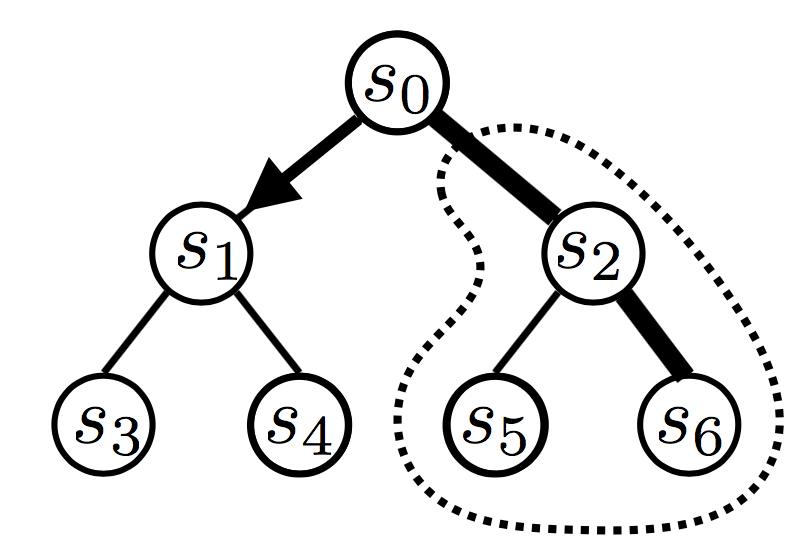
\includegraphics[trim={1cm 0.5cm 0 1cm},clip, width=0.22\textwidth]{./figure/binary_tree_MDP}
  \caption{The binary tree structure MDP $\tilde{\mathcal{M}}$. Under realizable and deterministic setting (see the text in Sec.~\ref{sec:special_mdp} for details), once the algorithm explores the right-most path (bold black) and learns that $Q^e(s_0, a_l)>Q^e(s_0,a_r)$ ($a_l$ denotes go-left action), it will not have to explore the right sub-tree (dot circle).}
  \label{fig:binary_MDP}
  \vspace{-5pt}
\end{figure}
We analyze the performance of general imitation learning (i.e., learning with access to $Q^e$). The goal is to demonstrate teh intuition that IL learns faster than RL. To measure the speed of learning, we use the \emph{cumulative} regret of the entire learning process, defined as $R_N = \sum_{n=1}^N (\mu(\pi^e) - \mu(\pi_n))$. A smaller regret rate of $R_N$ indicates faster learning. Below we will only show this result on discrete MDPs. Throughout this section, we assume the expert $\pi^e$ is optimal. We consider finite-horizon, episodic IL and RL algorithms. 


\subsection{A Special MDP}
\label{sec:special_mdp}
In Fig.~\ref{fig:binary_MDP}, we consider a $K$-depth binary tree-structured MDP $\tilde{\mathcal{M}}$ with $2^K-1$ states, and two actions ${a_l, a_r}$:  go-left and go-right. The transition is deterministic and the initial state $s_0$ is fixed. Note that there are only $2^{K-1}$ possible trajectories. The reward for each non-leaf state is zero, and the reward for each leaf is always i.i.d sampled from a given distribution (possibly different distributions for different leafs).  $S$ is the number of total states in $\tilde{\mathcal{M}}$ ($S = 2^K-1$). The following theorem shows the lower bound of $R_N$ for any finite-horizon, episodic RL algorithm on $\tilde{\mathcal{M}}$:
\begin{theorem}
\label{them:special_lower}
For the MDP $\tilde{\mathcal{M}}$, there exists a set of reward distributions for leaves such that  the regret $R_N$ of any finite-horizon ($H=K$), episodic RL algorithm is at least:
\begin{align}
\mathbb{E}[R_N] \geq \Omega(\sqrt{SN}),
\end{align} 
\end{theorem} where the expectation is with respect to random generation of rewards and internal randomness of the algorithm. Note that $S = 2^K-1$ in $\tilde{\mathcal{M}}$.
However, with the access to the expert's state-action value function $Q^e$, we show that there exists a policy class representation such that imitation learning can learn exponentially faster:% gives the following upper bound:
\begin{theorem}
\label{them:special_upper}
For the MDP $\tilde{\mathcal{M}}$, there exists an imitation learning algorithm (AggreVaTe with FTL) that can achieve the following regret bound:
\begin{align}
R_N \leq O(\log{S}).
\end{align}
\end{theorem}
Fig.~\ref{fig:binary_MDP} illustrates the intuition behind the theorem. During the first episode, the initial policy $\pi_1$ picks the rightmost trajectory (bold black) to explore. Once the algorithm receives a reward-to-go vector $[Q^e(s_0,a_l),Q^e(s_0,a_r)]$ for $s_0$ (assume $Q^e(s_0,a_l)>Q^e(s_0,a_r)$), it immediately learns that the optimal policy will go left (black arrow) at $s_0$. Hence the algorithm eliminates the entire right sub-tree (dot circle).


Next we consider the more difficult setting where one can only query for a noisy but unbiased estimate of $Q^e$. The above halving argument will not apply since deterministically eliminating nodes based on noisy estimates of the reward-to-go might permanently remove good trajectories. However, imitation learning can still achieve the reasonable regret, even in the noisy setting:
\begin{theorem}
\label{them:special_lower_noisy}
With only access to unbiased estimate of $Q^e$, for the MDP $\tilde{\mathcal{M}}$, there exists an imitation learning algorithm (AggreVaTe with EG) that can achieve the following regret with probability at least $1-\delta$:
\begin{align}
R_N \leq O\Big(\ln(S)(\sqrt{\ln(S)N}+\sqrt{\ln(2/\delta)N})\Big)
\end{align}
\end{theorem} In other words, imitation learning can still achieve a regret bound that is \emph{polylog} on the number of total states. The detailed proofs of the above three theorems can be found in Appendix~\ref{sec:special_lower},\ref{sec:special_upper},\ref{sec:proof_special_noisy} respectively. %The above results shows that for $\tilde{\mathcal{M}}$, imitation learning 
%To prove the lower bound shown in Theorem~\ref{them:special_lower}, we show that any Multi-Arm Bandits (MAB) problem can be reduced to $\tilde{\mathcal{M}}$ and it is well known that for stochastic MAB the lower bound of regret is $\Omega(KT)$, where $K$ is the number of arms 
In summary, for MDP $\tilde{\mathcal{M}}$, imitation learning is exponentially faster than RL. 

\subsection{General MDPs}
We next consider general discrete finite MDPs in the difficult case where we can only access an unbiased estimate of $Q^e_t$, for any $t$ and state-action pair. The policy $\pi$ is represented as a set of probability vectors $\pi^{s,t}\in\Delta(A)$, for all $s \in\mathcal{S}$ and  $t\in[H]$: $\pi = \{\pi^{s,t}\}_{s\in\mathcal{S},t\in[H]}$. 

%Namely it is possible that the policy, including $\pi^e$, at different state $s$ and different time step $t$ may has completely different action selection strategies.  

\begin{theorem}
\label{them:upper_bound}
With access to unbiased estimates of $Q^e_t$, AggreVaTe with EG achieves the regret upper bound:
\begin{align}
\label{eq:regret_eg}
R_N \leq O\big(HQ_{\max}^e\sqrt{S\ln(A)N}\big).
\end{align}
\end{theorem}
The advantage of using EG over OGD in dicrete MDPs comes from the almost dimension-free property of EG: $R_N$ only depends on $\sqrt{\ln(A)}$ instead of $\sqrt{A}$ which will appear in $R_N$ if one simply runs OGD on the sequence of losses $\ell_n(\pi)$. The total regret shown in Eq.~\ref{eq:regret_eg} allows us to compare IL algorithms to RL algorithms on discrete MDPs. For example, the Upper Confidence Bound (UCB) based, near-optimal optimistic RL algorithms from \cite{jaksch2010near}, specifically designed for efficient exploration, admit regret $\tilde{O}(HS\sqrt{H AN})$, leading to a gap of approximately $\sqrt{HAS}$ compared to the regret bound of imitation learning shown in Eq.~\ref{eq:regret_eg}. We also provide a lower bound on $R_N$ for $H=1$ case which shows the dependencies on $N, A, S$ are tight:
\begin{theorem}
\label{them:lower_bound}
There exists MDP with $H = 1$, with only access to unbiased estimate of $Q^e$, any finite-horizon episodic imitation learning algorithm  must have:
\begin{align}
\mathbb{E}[R_N] \geq \Omega(\sqrt{S\ln({A})N}).
\end{align}
\end{theorem} The proofs of the above two theorems regarding general MDPs can be found at Appendix~\ref{sec:proof_upper_bound},\ref{sec:proof_lower_bound}






\section{Experiments}
\begin{figure*}[t!]
	\centering
	\vspace{-2mm}
	\begin{subfigure}[l]{0.1962\textwidth}
        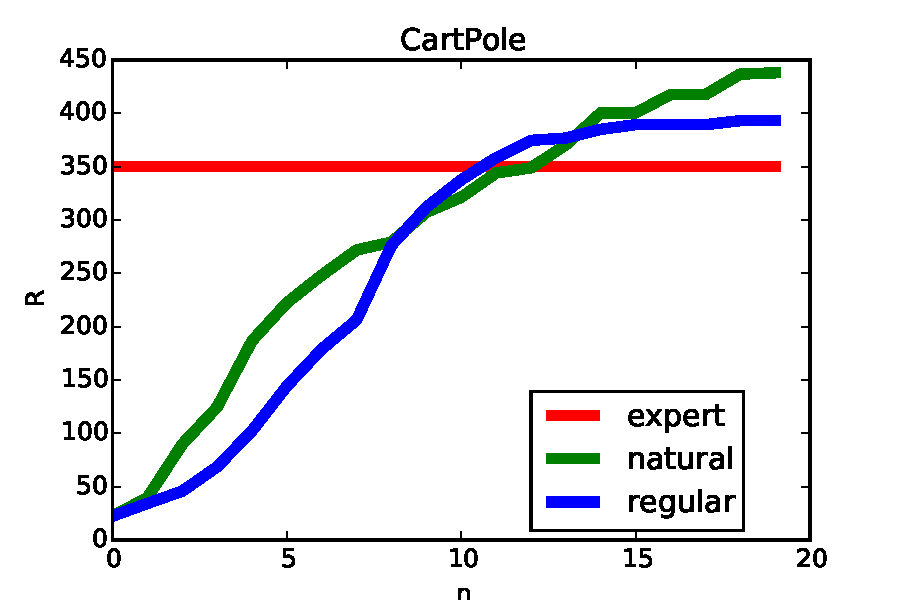
\includegraphics[width=1.12\textwidth,keepaspectratio]{./figure/CartPole_comparison.pdf}
        \caption{Cartpole}
        \label{fig:cartpole}
    \end{subfigure}
    %\end{subfigure}
	\begin{subfigure}[l]{0.1962\textwidth}
        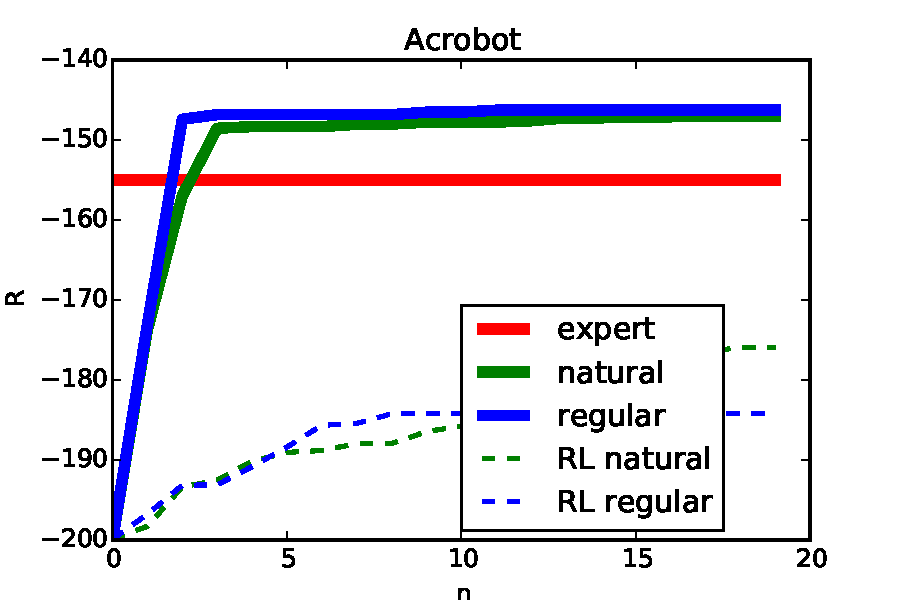
\includegraphics[width=1.12\textwidth,keepaspectratio]{./figure/Acrobot_comparison_200.pdf}
        \caption{Acrobot}
        \label{fig:acrobot}
    \end{subfigure}
    \begin{subfigure}[l]{0.1962\textwidth}
        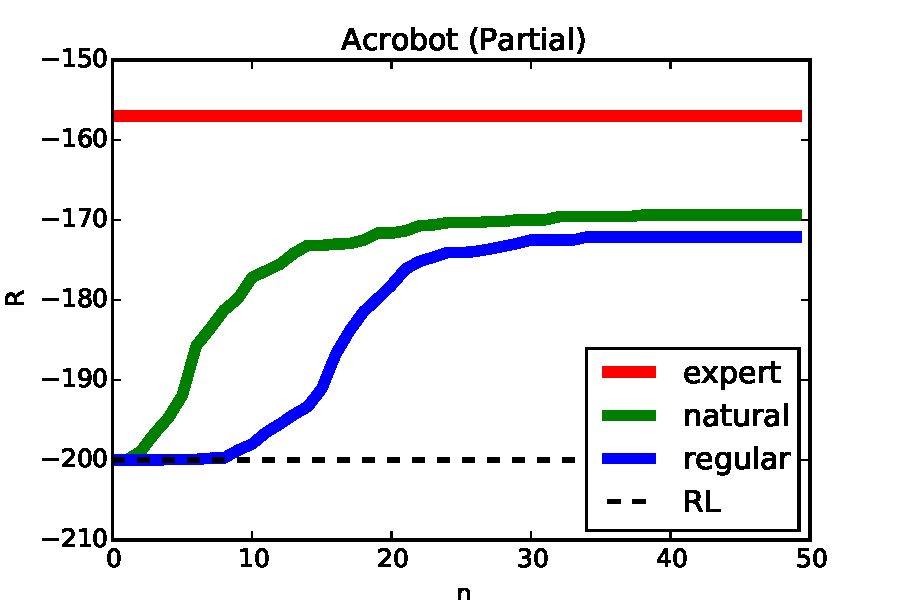
\includegraphics[width=1.12\textwidth,keepaspectratio]{./figure/Acrobot_LSTM_comparison.pdf}
        \caption{Acrobot (POMDP)}
        \label{fig:acrobot_partial}
    \end{subfigure}
    \begin{subfigure}[l]{0.1962\textwidth}
        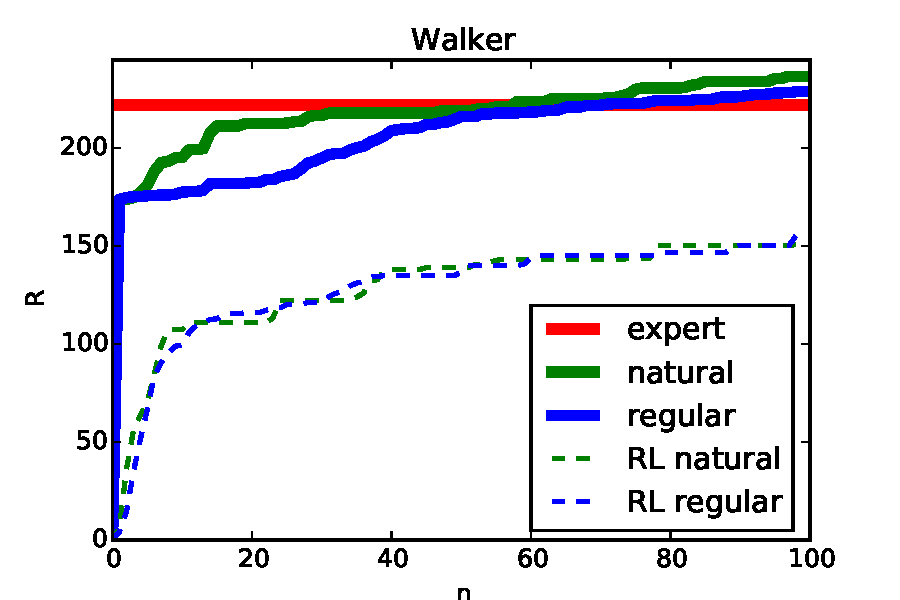
\includegraphics[width=1.12\textwidth,keepaspectratio]{./figure/Walker_comparison.pdf}
        \caption{Walker}
        \label{fig:walker}
    \end{subfigure}
    %\end{subfigure}
	\begin{subfigure}[l]{0.1962\textwidth}
        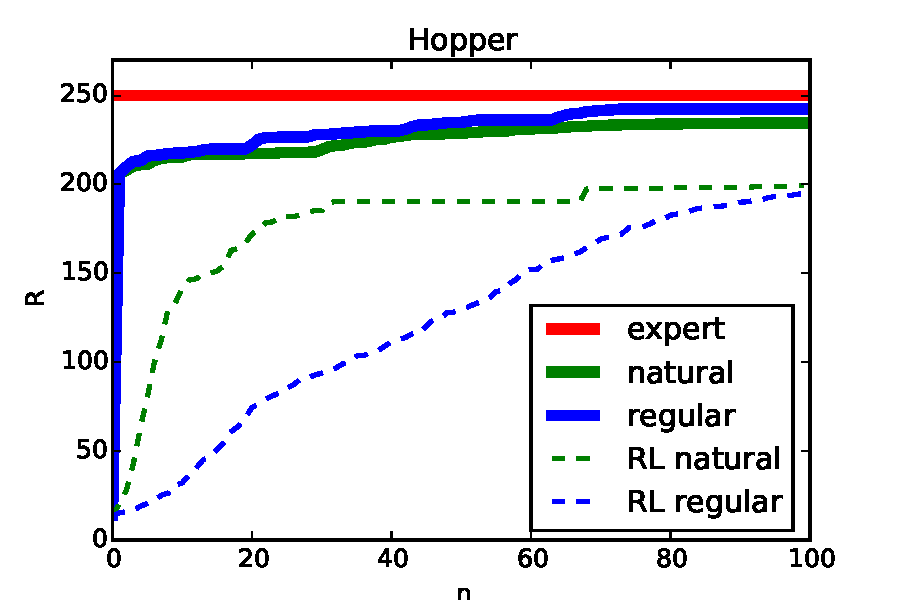
\includegraphics[width=1.12\textwidth,keepaspectratio]{./figure/Hopper_comparison.pdf}
        \caption{Hopper}
        \label{fig:hopper}
    \end{subfigure}
    \caption{Performance ($R_n$ on y-axis) versus number of iterations ($n$ on x-axis) of DIL (blue and green), experts (red), and RL algorithms (dotted) on different robotics simulators. }
    \label{fig:perf_robotics}
\end{figure*}
We evaluate our algorithms on robotics simulations from OpenAI Gym \cite{brockman2016openai} and on Handwritten Algebra Dependency Parsing \cite{duyckpredicting}. Since our approach, in theory, promises that there exists a policy among all of the learned polices that can perform as well as the expert, we report the performance of the best policy so far: $R_i = \max\{\mu(\pi_1), ..., \mu(\pi_i)\}$. For both IL and RL, for regular gradient ascent, we use ADAM \cite{kingma2014adam} which itself is a first-order no-regret online algorithm, and for natural gradient ascent, we use Conjugate Gradient with fixed number of iterations (aka Truncated Natural Gradient \cite{duan2016benchmarking}) to compute the ascent direction. 


\subsection{Robotics Simulations}
For the discrete action setting we consider the CartPole balancing task and Acrobot Swing-up task. For the continuous action setting we consider the Hopper and the Walker. For the purpose of generating an expert, similar to previous work \cite{ho2016generative}, we implemented a Deep Q-Network (DQN) to generate $Q^e$ for the CartPole and the Acrobot (e.g., to simulate the settings where $Q^e$ is available), while using the public available TRPO implementation to generate $\pi^e$ for continuous tasks to simulate the settings where one needs to estimate $Q^e$ by Monte-Carlo roll outs $\pi^e$. %In order to demonstrate DIL's ability to outperform experts, we did not run DQN or TRPO for large amount of time nor tune the parameters extremely hard to get $\pi^e$ or $Q^e$. 



\paragraph{Discrete Action Setting} Cart-Pole and Acrobot have discrete actions. We use a one-layer (16 hidden units) neural network with ReLu activation functions to represent the policy $\pi$. The value function $Q^e$ is obtained from the DQN \cite{mnih2015human} and represented by a multi-layer fully connected neural network. The policy $\pi_{\theta_1}$ is initialized by the common ReLu neural network initialization techniques. For scheduling rate $\{a_i\}$, we set all $a_i = 0$: we neither asked for nor executed the expert's actions during training. We set the number of roll outs $K = 50$ and horizon $H = 500$ for the cartpole and $H = 300$ for the acrobot.



Fig.~\ref{fig:cartpole} and \ref{fig:acrobot} shows the performance averaged over 10 random trials of DIL with regular gradient ascent and natural gradient ascent. Note that DIL outperforms the experts' performance significantly: Natural gradient surpass experts 5.8$\%$ in Acrobot and $\mathbf{25\%}$ in Cart-pole. Also, for Acrobot swing-up, at horizon $H=300$, with high probability a random neural network policy won't be able to collect any reward signals. Hence the improvement rate of REINFORCE and Truncated Natural Gradient is slow. In fact, we observed that for a short horizon such as $H=300$, REINFORCE and Truncated Natural Gradient often even fail to improve the policy at all (failed 6 times among 10 trials). On the contrary, DIL will not suffer from the delayed reward signal issue, since the expert will collect reward signals much faster than a random policy. 

In Acrobot partially-observable setting (observations are the positions of the links), Fig.~\ref{fig:acrobot_partial} shows the performance of DIL with an LSTM policy (32 hidden states) where the expert has access to full states but the learner can only access to observations. We make the problem harder by setting $H=200$. RL algorithms did not achieve any improvement while DIL still achieves 92$\%$ of expert's performance.

\paragraph{Continuous Action Setting}
We test our approaches on two robotics simulators with continuous actions: (1) the 2-d Walker and (2) the Hopper from the MuJoCo physics simulator. Following the neural network settings described in \citet{schulman2015trust}, the expert policy $\pi^e$ is obtained from TRPO with one hidden layer (64 hidden states), which is the same structure that we use to represent our policies $\pi_{\theta}$. We set $K = 50$ and $H = 100$. We initialize $\pi_{\theta_1}$ by collecting $K$ expert demonstrations and then maximize the likelihood of these demonstrations. We use Eq.~\ref{eq:gradient_finite_con} instead of the variance reduced equation here since we need to use MC roll-outs to estimate $V^e$ (we simply use one roll-out to estimate $Q^e$). %which will introduce more variance.


Fig.~\ref{fig:walker} and \ref{fig:hopper} show the performance averaged over 5 random trials. Note that DIL significantly outperforms the expert in the Walker problem while achieving 97$\%$ of the expert's performance in the Hopper problem. After 100 iterations, we see that by leveraging the help from experts, DIL can achieve much faster improvement rate than the corresponding RL algorithms. 


\subsection{Dependency Parsing on Handwritten Algebra}
\begin{table*}[t!]
\begin{center}
\resizebox{1.\textwidth}{!}{ 
    %\begin{tabular}{| l | l | l | l | l | l| l| l| }
    \begin{tabular}{llllllllllr}
   \toprule
    Arc-Eager & DIL (LSTMs)   & DIL (NN)   & SL-RL (LSTMs) & SL-RL(NN) & RL (LSTMs) & RL (NN) & DAgger & SL (LSTMs) & SL (NN) & Random \\ 
    \midrule
    \textbf{Regular} & \textbf{0.924}$\pm$0.10 & 0.851$\pm$0.10 & 0.826$\pm$ 0.09& 0.386$\pm$0.1 & 0.256$\pm$0.07 & 0.227$\pm$0.06 & \multirow{2}{*}{0.832$\pm$0.02} & \multirow{2}{*}{0.813$\pm$0.1} 
    & \multirow{2}{*}{0.325$\pm$0.2}
    &\multirow{2}{*}{$\sim$0.150}\\
    
    \textbf{Natural} & 0.915$\pm$0.10 & 0.800$\pm$0.10 & 0.824$\pm$0.10 & 0.345$\pm$0.1 & 0.237$\pm$0.07 &0.241$\pm$0.07 \\
    %\textbf{Mean} &  21183.3$\pm$1263.1 & {31716.5$\pm$1016.0} \\ 
    %\textbf{GCR} & 33712.5$\pm$1852.1 &  48195.7$\pm$1952.7 \\ 
    \bottomrule
    %\textbf{Flag Video Texture} & 1.28e3$\pm$7.1e1 & 1.63e3$\pm$9.7e1  & \textbf{1.24e3$\pm$9.6e1} \\ \hline
    \end{tabular}}
\end{center}
\vspace{-5pt}
\caption{Performance (Unlabeled Attachment Score) of different approaches on handwritten algebra dependency parsing. \emph{SL} stands for supervised learning using expert's samples: maximizing the likelihood of expert's actions under the sequences generated by expert itself. \emph{SL-RL} means RL with initialization using SL. \emph{Random} stands for the initial performances of random policies (LSTMs and NN).
The performance of DAgger with Kernel SVM is from \cite{duyckpredicting}.} %and Forward Training and SMILe \cite{ross2010efficient} performed worse than DAgger.}
\label{tab:eager}
\end{table*}

We consider a structured prediction problem: transition-based dependency parsing for handwritten algebra with raw-pixel image data \cite{duyckpredicting}. The parsing task for algebra is similar to the classic dependency parsing for natural language \cite{chang2015learning_dependency} where the problem is modelled as imitation learning setting and the state-of-the-art result is achieved by AggreVaTe using Data Aggregation (FTL or FTRL). The additional challenge here is that the inputs are handwritten algebra symbols in raw-pixel images. Following suggestions from \cite{duyckpredicting}, we directly learn to predict dependency trees from low level image features (Histogram of Gradient features (HoG)). The expert is constructed using the ground-truth dependencies in the training data\footnote{In configurations which have multiple optimal transitions, our implementation of expert picks the first action deterministically in the order of Shift, Right, Left, Reduce.}. The full state $s$ during parsing consists of three data structures: stack, buffer and arcs, which all store raw images of the algebraic symbols. Since the sizes of stack, buffer and arcs are changing during parsing, common approach to featurize the state $s$ is to take the features of the latest three symbols from stack, buffer and arcs (e.g., \cite{chang2015learning_dependency}). Hence the problem falls into the \emph{partially observable} setting, where the feature $o$ is extracted from state $s$ and only contains partial information about $s$. %Hence this problem can be considered as imitation learning in partial observable setting.
The dataset consists of 400 sets of handwritten algebra equations. We use 80$\%$ for training, 10$\%$ for validation, and 10$\%$ for testing. We include an example of handwritten algebra equations and its dependency tree in Appendix~\ref{sec:parsing_example}. Note that different from robotics simulators where every episode one can get freshly new data from simulators, here the size of dataset is fixed and the sample efficiency is even more critical. 

The recurrent neural network policy that we used follows the design from \cite{sutskever2014sequence}: the RNN policy consists of two LSTMs: given a sequence  of algebra symbols $\tau$, the first LSTM goes through $\tau$ one symbol at a time and at the end of the sequence outputs its hidden states and memory (i.e., as a summary of $\tau$).The second LSTM then initializes its own hidden states and memory using the outputs of the first LSTM. At every parsing step $t$, the second LSTM takes the current partial observation $o_t$ ($o_t$ consists of features of the most recent item from stack, buffer and arcs) and action $a_t$ as inputs, and uses its internal hidden state and memory to compute the policy $\pi(\cdot|o_1,...,o_t,\tau)$ conditioned on the whole history. We also tested reactive policies which are represented by fully connected ReLu neural networks (NN) (one-layer with 1000 hidden states) that directly maps from observation $o$ to action $a$, where $o_t$ uses the most three recent items from stack, buffer and arcs. We use variance reduced gradient estimations, which give better performance. The performance is summarised in Table~\ref{tab:eager}. Due to the partial observability property of the problem setting, DIL with LSTM policy achieves significantly better UAS scores compared to NN based policy and DAgger with Kernel SVM \cite{duyckpredicting}. Also DIL with LSTM policy achieves 97$\%$ of optimal expert's performance. Fig.~\ref{fig:perf_eager} shows the improvement rate of regular gradient ascent and natural gradient ascent on both validation set and test set. Overall we observe that both methods have similar performance. Natural gradient ascent achieves better UAS score in validation set and converges slightly faster on test set but achieves lower UAS score in test set. 


%\begin{table}[t]
%\begin{center}
%    \begin{tabular}{| l | l | l | l | l| l| }
%    \hline
%      Acr-Hybird & NN (1000)  & NN (200+20) & LSTM (50) \\ \hline
%    {RL} & / &  / & / \\ 
%    \hline 
%    {DIL} & / & / & / \\ 
%    \hline
%    \hline
%     Arc-Eager & NN (1000)  & NN (200+20) & LSTM (50) \\ \hline
%    {RL} & / &  / & / \\ 
%    \hline 
%    {DIL} & / & / & / \\ 
%    \hline
%\end{tabular}
%\end{center}
%\caption{Performance of DIL with regular gradient ascent on handwritten algebra dependency parsing for different policy representations: one layer NN with 1000 hidden states, two-layer NN with 200 and 20 hidden states in the first and second layer respectively, and RNN policy that consists of two LSTMs with 50 hidden states. 
%}
%\label{tab:hybird}
%\end{table}


\begin{figure}[t!]
	\centering
	\vspace{-2mm}
	\begin{subfigure}[l]{0.238\textwidth}
        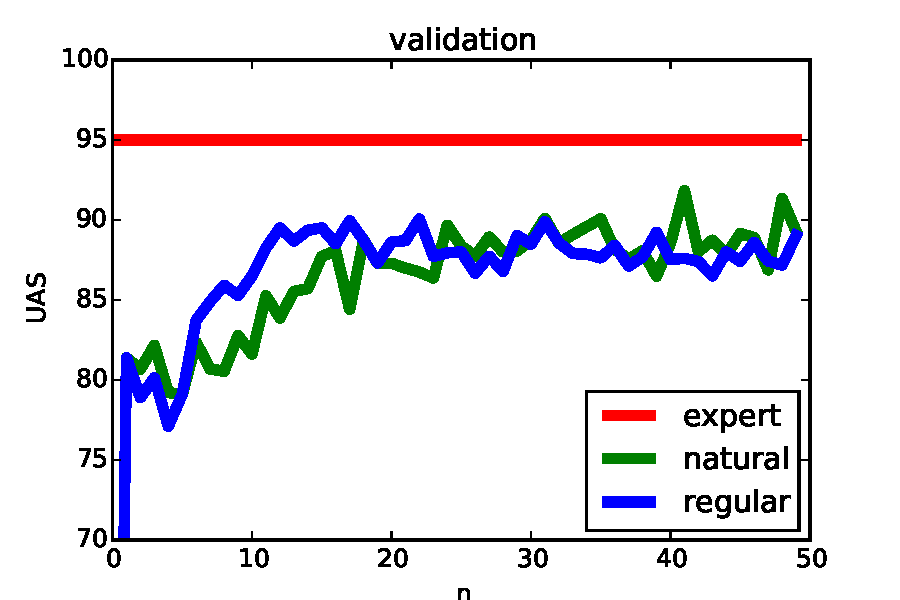
\includegraphics[width=1.11\textwidth,keepaspectratio]{./figure/eager_validation_comparison.pdf}
        \caption{Validation}
        \label{fig:cartpole}
    \end{subfigure}
    %\end{subfigure}
	\begin{subfigure}[l]{0.238\textwidth}
        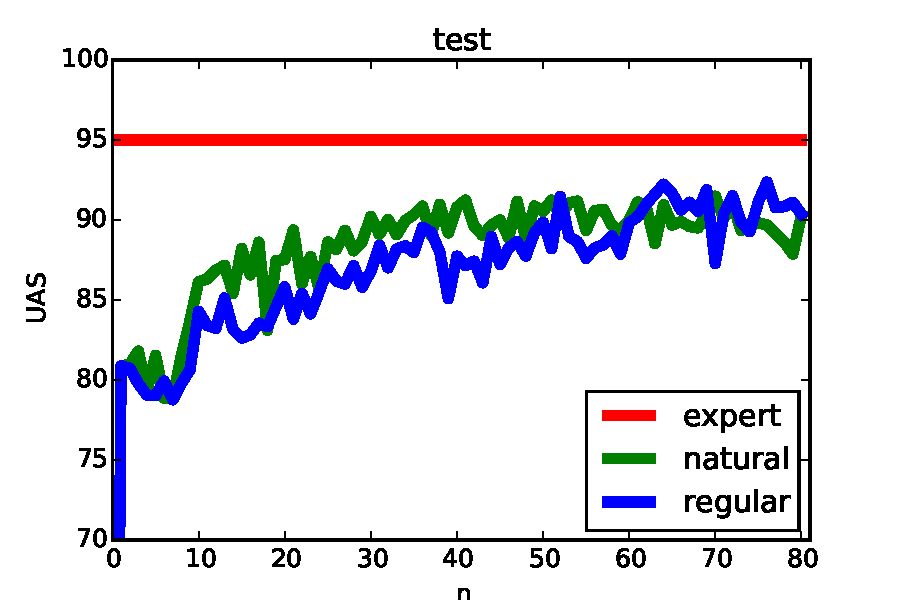
\includegraphics[width=1.11\textwidth,keepaspectratio]{./figure/eager_test_comparison_2.pdf}
        \caption{Test}
        \label{fig:acrobot}
    \end{subfigure}
    \caption{UAS (y-axis) versus number of iterations ($n$ on x-axis) of DIL with LSTM policy (blue and green), experts (red) on validation set and test set for Arc-Eager Parsing. }
    \label{fig:perf_eager}
\end{figure}



\section{Conclusion}
We present a framework that shows how policy gradient methods can be used for imitation learning and structured prediction. Closely following the reduction framework from \citet{ross2014reinforcement}, we present a regular gradient ascent procedure that integrates ordinary gradient ascent as the no-regret learner with AggreVaTe, and a natural gradient ascent procedure motivated from the integration of EG with AggreVaTe. Our differentiable imitation learning algorithm enables us to train complicated non-linear polices (e.g., neural network polices) efficiently on challenging tasks ranging from high-dimensional continuous robotics control to dependency parsing on raw image data. We empirically show that the policies learned by our method exhibit similar performance to optimal experts and sometimes can learn to perform better than experts that only provide suboptimal trajectories to the learner. In addition to these empirical results, we also provide a theoretical study of the learning efficiency of IL and show that IL is much more sample efficient compared with RL algorithms. This suggests that, when expert advice is available, one should use IL instead of RL to learn policies.
%$, which matches to the original analysis of AggreVaTe. 


%Our work opens the possibilities of using state-of-art policy gradient methods developed from Deep Reinforcement Learning literature to advance imitation learning and structured prediction. One interesting future work 

%One interesting future work is to apply Trust Region Policy Optimization (TRPO) \cite{schulman2015trust} to imitation learning and structured prediction, though TRPO usually demonstrates similar performance as natural gradient methods \cite{duan2016benchmarking}. Another interesting direction is to apply DIL to LOLS \cite{chang2015learning} which additionally guarantees local optimality in the case of sub-optimal experts. 


\vspace{-5pt}

%\section*{Acknowledgements}
%\vspace{-5pt}
%This material is based upon work supported in part by: DARPA ALIAS contract number HR0011-15-C-0027 and National Science Foundation Graduate Research Fellowship Grant No. DGE-1252522. The authors also thank Geoff Gordon for valuable discussions.





{\small
\bibliography{reference}
\bibliographystyle{icml2016}
}


\newpage
\onecolumn
\appendix
\paragraph{Appendix: Proofs and Detailed Bounds}

\section{Derivation of Exponential Gradient Update in Discrete MDP}
\label{sec:EG_derivation}
We show the detailed derivation of Eq.~\ref{eq:eg_closed_form} for AggreVaTe with EG in discrete MDP. Recall that with $KL$-divergence as the penalization, one update the policy in each episode as:
\begin{align}
\{\pi_{n+1}^s\}_{s\in\mathcal{S}} &= \arg\max_{\{\pi^s\in \Delta(A),\forall s\}}\frac{1}{H}\sum_{t=1}^H\sum_{s\in\mathcal{S}}d_t^{\pi_n}(s)\big( \pi^s\cdot Q_t^e(s)\big) - \sum_{s\sim\mathcal{S}}\frac{\bar{d}^{\pi_n}(s)}{\mu_{n,s}}KL(\pi_s \| \pi_n^s) \nonumber
\end{align} Note that in the above equation, for a particular state $s$, optimizing $\pi^s$ is in fact independent of $\pi^{s'}, \forall s'\neq s$. Hence the optimal sequence $\{\pi^s\}_{s\in\mathcal{S}}$ can be achieved by optimizing $\pi^s$ independently for each $s\in\mathcal{S}$. For $\pi^s$, we have the following update rule:
\begin{align}
\pi_{n+1}^s = &\arg\max_{\pi^s\in\Delta(A)}\frac{1}{H}\sum_{t=1}^H d_t^{\pi_n}(s)(\pi^s\cdot Q^e_t(s)) - \frac{\bar{d}^{\pi_n}(s)}{\mu_{n,s}}KL(\pi_s\| \pi_n^s) \nonumber\\
& = \arg\max_{\pi^s\in\Delta(A)}\pi^{s}\cdot (\sum_{t=1}^H d_t^{\pi_n}(s)Q_t^e(s) / H) - \frac{\bar{d}^{\pi_n}(s)}{\mu_{n,s}}KL(\pi_s\|\pi_n^s) \nonumber\\
& = \arg\max_{\pi^s\in\Delta(A)}\pi^{s}\cdot (\sum_{t=1}^H d_t^{\pi_n}(s)Q_t^e(s) /(H\bar{d}^{\pi_n}(s))) - \frac{1}{\mu_{n,s}}KL(\pi_s\|\pi_n^s) \nonumber\\
& = \arg\max_{\pi^s\in\Delta(A)}\pi^s\cdot \tilde{Q}^e(s) - \frac{1}{\mu_{n,s}}\sum_{j=1}^A \pi^s[j](\log(\pi^s[j]) - \log(\pi_n^s[j]))
\end{align} Take the derivative with respect to $\pi^s[j]$, and set  it to zero, we get:
\begin{align}
\tilde{Q}^e(s)[j] -\frac{1}{\mu_{n,s}}(\log(\pi^s[j]/\pi_n^s[j]) + 1) = 0,
\end{align} this gives us:
\begin{align}
\pi^s[j] = \pi_n^s[j]\exp(\mu_{n,s}\tilde{Q}^e(s)[j]-1).
\end{align} Since $\pi^s\in\Delta(A)$, after normalization, we get:
\begin{align}
\pi^s[j] = \frac{\pi_n^s[j]\exp(\mu_{n,s}\tilde{Q}^e(s)[j])}{\sum_{i=1}^A \pi_n^s[i]\exp(\mu_{n,s}\tilde{Q}^e(s)[i])}
\end{align}



\section{Lemmas}
Before proving the theorems, we first present the \emph{Performance Difference Lemma} \cite{kakade2002approximately,ross2014reinforcement} which will be used later:
\begin{lemma}
\label{lemma:performance_difference}
For any two policies $\pi_1$ and $\pi_2$, we have:
\begin{align}
\mu(\pi_1) - \mu(\pi_2) = H\sum_{t=1}^H \mathbb{E}_{s_t\sim d_t^{\pi_1}}\big[\mathbb{E}_{a_t\sim \pi_1(\cdot|s_t)}[Q_t^{\pi_2}(s_t,a_t) - V_t^{\pi_2}(s_t)]\big].
\end{align}
\end{lemma} We refer readers to \cite{ross2014reinforcement} for the detailed proof of the above lemma. 

The second known result we will use is the analysis of Weighted Majority Algorithm. Let us define the linear loss function as $\ell_n(w) = w\cdot y_n$, for any $y_n\in\mathbb{R}^d$, and $w\in\Delta(d)$ from a probability simplex. Running Exponential Gradient Algorithm on the sequence of losses $\{w\cdot y_n\}$ to compute a sequence of decisions $\{w_n\}$, we have:
\begin{lemma} 
\label{lemma:EG}
The sequence of decisions $\{w_n\}$ computed by running Exponential Gradient Ascent with step size $\mu$ on the loss functions $\{w\cdot y_n\}$ has the following regret bound:
\begin{align}
\max_{w^*\in\Delta(d)} \sum_{n=1}^N (w^*\cdot y_n - w_n\cdot y_n) \leq \frac{\ln(d)}{\mu} + \frac{\mu}{2}\sum_{n=1}^N\sum_{i=1}^d w_n[i] y_n[i]^2.
\end{align}
\end{lemma} We refer readers to \cite{shalev2012online} for detailed proof.


\section{Proof of Theorem~\ref{them:special_lower}}
\label{sec:special_lower}
\begin{proof}
We construct a reduction from stochastic Multi-Arm Bandits (MAB) to the MDP $\tilde{\mathcal{M}}$. A stochastic MAB is defined by $S$ arms denoted as $I^1, ..., I^S$. Each arm $I^t$'s reward $r_{i}$ at any time step $t$ is sampled from a fixed but unknown distribution. A bandit algorithm picks an arm $I_t$ at  iteration $t$ and then receives an unbiased sample of the picked arm's reward $r_{I_t}$. For any bandit algorithm that picks arms $I_1, I_2,...,I_N$ in $N$ rounds, the expected regret is defined as:
\begin{align}
\mathbb{E}[R_N] = \max_{i\in [S]}\sum_{n=1}^N \bar{r}_{i} - \mathbb{E}[  \sum_{n=1}^N r_{I_n}],
\end{align} where the expectation is taken with respect to the randomness of the reward sampling process and possibly the randomness of the bandit algorithm. It has been shown that there exists a set of Bernoulli distributions from which the arms' rewards sampled from, the expected regret $\mathbb{E}[R_N]$ is at least $\Omega(\sqrt{S N})$. 

Consider a MAB with $2^{K}$ arms. To construct a MDP from a MAP, we construct a $K+1$-depth binary-tree structure MDP with $2^{K+1}-1$ nodes. We set each node in the binary tree as a state in the MDP. The number of actions of the MDP is two, which corresponds to go left or right at a node in the binary tree. We associate each leaf nodes with arms in the original MAB: the reward of the $i$'th leaf node is sampled from the reward distribution for the $i$'th arm, while the non-leaf nodes have reward always equal to zero. The initial distribution $\rho_0$ concentrates on the root of the binary tree. Note that there are total $2^K$ trajectories from the root to leafs, and we denote them as $\tau_1,...\tau_{2^K}$. We consider finite horizon ($H=K+1$) episodic RL algorithms that outputs $\pi_1,\pi_2,...,\pi_N$ at $N$ episodes, where $\pi_n$ is any deterministic policy that maps a node to actions \emph{left} or \emph{right}. Any RL algorithm must have the following regret lower bound:
\begin{align}
\label{eq:bandit_to_RL}
\max_{\pi^*}\sum_{n=1}^N \mu(\pi^*) - \mathbb{E}[\sum_{n=1}^N \mu(\pi_n)] \geq \Omega(\sqrt{SN}),
\end{align} where the expectation is taken with respect to the possible randomness of the RL algorithms. Note that any deterministic policy $\pi$ identifies a trajectory in the binary tree when rolling in from the root. The optimal policy $\pi^*$ simply corresponds to the trajectory that leads to the leaf with the maximum expected reward. Note that each trajectory is associated with an arm from the original MAB, and the expected total reward of a trajectory corresponds to the expected reward of the associated arm. Hence if there exists an RL algorithm that achieves regret less than $O(\sqrt{SN})$, then we can solve the original MAB problem by simply running the RL algorithm on the constructed MDP. Since the lower bound for MAB is $\Omega(\sqrt{SN})$, this concludes that Eq.~\ref{eq:bandit_to_RL} holds. 
\end{proof}

\section{Proof of Theorem~\ref{them:special_upper}}
\label{sec:special_upper}
\begin{proof}
For notation simplicity we denote $a_l$ as the go-left action while $a_r$ is the go-right action. Without loss of generality, we assume that the leftmost trajectory has the highest total reward (e.g., $s_3$ in Fig.~\ref{fig:binary_MDP} has the highest average reward).
We consider the deterministic policy class $\Pi$ that contains all policy $\pi: \mathcal{S}\to \{a_l,a_r\}$. Since there are $S$ states and 2 actions, the total number of policies in the policy class is $2^S$. To prove the upper bound $R_N\leq O(\log(S))$, we claim that for any $e\leq K$, at the end of episode $e$, AggreVaTe with FTL identifies the $e$'th state on the best trajectory, i,e, the leftmost trajectory $s_0, s_1, s_3, ..., s_{(2^{K-1}-1)}$. We can prove the claim by induction. 

At episode $e=1$, based on the initial policy, AggreVaTe picks a trajectory $\tau_1$ to explore. %Denote the trajectory as $s_0, s^{1,1}, ..., s^{1,k}$, where $s^{e,t}$ represents the state that is visited at episode $e$, at time step $t$. 
AggreVaTe with FTL collects the states $s$ at $\tau_1$ and their associated reward-to-go vectors $[Q^e(s,a_l), Q^e(s,a_r)]$. Let us denote $D_1$ as the dataset that contains the state,reward-to-go pairs: $D_1 = \{(s, [Q^e(s,a_l),Q^e(s,a_l)])\}$, for $s\in \tau_1$. Since $s_0$ is visited, the state-cost pair $(s_0, [Q^e(s_0,a_l),Q^e(s_0,a_r)])$ must be in $D_1$. To update policy from $\pi_1$ to $\pi_2$, AggreVaTe with FTL runs cost-sensitive classification $D_1$ as:
\begin{align}
\label{eq:cs}
\pi_2 = \arg\max_{\pi}\sum_{k=1}^{|D_1|} Q^e(s_k, \pi(s_k)),
\end{align} where $s_k$ stands for the $k$'th data point collected at dataset $D_1$. Due to the construction of policy class $\Pi$, we see that $\pi_2$ must picks action $a_l$ at state $s_0$. Hence at the end of the episode $e=1$, $\pi_2$ identifies $s_1$, which is on the optimal trajectory.  

Now assume that at the end of episode $n-1$, the newly updated policy $\pi_{n}$ identifies the state $s_{(2^{n-1}-1)}$: namely at the beginning of episode $n$, if we roll-in $\pi_n$, the algorithm will keep traverse along the leftmost trajectory till at least state $s_{(2^{n-1}-1)}$. At episode $n$, let $D_n$ as the dataset contains all data points from $D_{n-1}$ and the new collected state, reward-to-go pairs from $\tau_n$: $D_n = D_{n-1}\cup \{(s, [Q^e(s,a_l),Q^e(s,a_r)])\} $, for all $s\in\tau_n$. Now if we compute policy $pi_{n+1}$ using cost-sensitive classification (Eq.~\ref{eq:cs}) over $D_n$, we must learn a policy $\pi_{n+1}$ that identifies action $a_l$ at state $s_{(2^{j}-1)}$, since $Q^{e}(s_{(2^{j}-1)}, a_l)> Q^e(s_{(2^{j}-1)}, a_r)$, and $s_{(2^j - 1)}$ is included in $Q_n$, for $j=1,..., n-1$.  Hence at the end of episode $n$, we identify a policy $\pi_{n+1}$ such that if we roll in policy $\pi_{n+1}$ from $s_0$, we will traverse along the left most trajectory till we reach $s_{(2^n-1)}$.  

Hence by the induction hypothesis, at the end of episode $K-1$, $\pi_{K}$ will reach state $s_{(2^{K-1}-1)}$, the end of the best trajectory.

Since AggreVaTe with FTL with policy class $\Pi$ identifies the best trajectory with at most $K-1$ episodes, the cumulative regret is then at most $O(K)$, which is $O(\log(S))$ (assuming the average reward at each leaf is a bounded constant), as $S$ is the number of nodes in the binary-tree structure MDP $\tilde{\mathcal{M}}$.
\end{proof}


\section{Proof of Theorem~\ref{them:special_lower_noisy}}
\label{sec:proof_special_noisy}
Since in Theorem~\ref{them:special_lower_noisy} we assume that we only have access to the noisy, but unbiased estimate of $Q^e$, the problem becomes more difficult since unlike in the proof of Theorem~\ref{them:special_upper}, we cannot simply eliminate states completely since the reward-to-go of the states queried from expert is noisy and completely eliminate nodes will potentially result elimination of high reward trajectories.  Hence here we consider a different policy representation. We define $2^{K}$ base policies $\pi^1, ..., \pi^{2^K}$, such that rolling in policy $\pi^i$ at state $s_0$ will traverse along the trajectory ending at the $i$'th leaf. We define the policy class $\Pi$ as the convex hull of the base policies $\Pi = \{\pi: \sum_{i=1}^{2^K}w_i\pi^i, \sum_i^{2^K}w_i = 1, w_i\geq 0, \forall i\}$. Namely each $\pi\in\Pi$ is a stochastic policy: when rolling in, with probability $w_i$, $\pi$ execute the $i$'th base policy $\pi^i$ from $s_0$. Below we prove that AggreVaTe with Exponential Gradient Ascent achieves the regret bound $O(\sqrt{\ln(S) N})$.



\begin{proof}
We consider finite horizon, episodic imitation learning setting where at each episode $n$, the algorithm can roll in the current policy $\pi_n$ once and only once and traverses through trajectory $\tau_n$ . Let us define $\tilde{\ell}_n(w) = \frac{1}{K+1}\sum_{t=1}^{K+1} \sum_{s\in\tau_n}\sum_{j=1}^{2^K}w_j \tilde{Q}^e(s,\pi^j(s))$, where $\tau_n$ is the trajectory traversed by rolling in policy $\pi_n$ starting at $s_0$, and $\tilde{Q}^e$ is a noisy but unbiased estimate of $Q^e$. We simply consider the setting where $\tilde{Q}^e$ is bounded $|\tilde{Q}^e| \leq l_{\max}$ (note that we can easily extend our analysis to a more general case where $\tilde{Q}^e$ is from a sub-Gaussian distribution). Note that $\tilde{\ell}_n(w)$ is simply a linear loss with respect to $w$:
\begin{align}
\tilde{\ell}_n(w) = w\cdot q_n,
\end{align} where $q_n[j] = \sum_{s\in\tau_n} \tilde{Q}^e(s,\pi^j(s))/(K+1)$. AggreVaTe with EG updates $w$ using Exponential gradient ascent. Using the result from lemma~\ref{lemma:EG}, we get:
\begin{align}
&\sum_{n=1}^N (\tilde{\ell}_n(w^*) - \tilde{\ell}_n(w)) = \sum_{n=1}^N (w^* \cdot q_n - w_n\cdot q_n) \leq \frac{\ln(2^K)}{\mu} + \frac{\mu}{2}\sum_{n=1}^N \sum_{j=1}^{2^K} w_n[j] q_n[j]^2 \leq \frac{\ln(2^K)}{\mu} + \frac{\mu}{2}\sum_{n=1}^N l_{\max}^2 \nonumber\\
& = \frac{\ln(2^K)}{\mu} + \frac{\mu N l_{\max}^2}{2} \leq l_{\max}\sqrt{\ln(S) N}.
\end{align} The above inequality holds for any $w^*\in \Delta(2^K)$, including the $w^e$ that corresponds to the expert (i.e., $w^e[1] = 1, w^e[i]=0,i\neq 1$ as we assumed without loss of generality the left most trajectory is the optimal trajectory).

Now let us define $\ell_n(w)$ as follows:
\begin{align}
\ell_n(w) = \frac{1}{K+1}\sum_{t=1}^{K+1}\sum_{s\sim \mathcal{S}} d_t^{\pi_n}(s)\sum_{j=1}^{2^K} w_j Q^e(s,\pi^j(s)).
\end{align} Note $\ell_n(w)$ can be understood as first rolling in $\pi_n$ \emph{infinitely many times} and then querying for the exact reward-to-go $Q^e$ on all the visited states. Clearly $\tilde{\ell}_n(w)$ is an unbiased estimate of $\ell_n(w)$: $\mathbb{E}[\tilde{\ell}_n(w)] -\ell_{n}(w) = 0$, where the expectation is over the randomness of the roll-in and sampling procedure of $\tilde{Q}^e$ at iteration $n$, conditioned on all events among the previous $n-1$ iterations. Also note that $|\tilde{\ell}_n(w) - \ell_n(w)| \leq 2l_{\max}$, since $\ell_n(w) \leq l_{\max}$. Hence $\{\tilde{\ell}_n(w_n) - \ell_n(w_n)\}$ is a bounded martingale difference sequence. Hence by Azuma-Heoffding inequality, we get with probability at least $1-\delta/2$:
\begin{align}
\sum_{n=1}^{N} \tilde{\ell}_n(w_n) - {\ell}_n(w_n) \leq 2l_{\max}\sqrt{\log(2/\delta)N},
\end{align} and with probability at least $1-\delta/2$:
\begin{align}
\sum_{n=1}^{N} {\ell}_n(w^e) - \tilde{\ell}_{n}(w^e) \leq 2l_{\max}\sqrt{\log(2/\delta)N}.
\end{align} Combine the above inequality using union bound, we get with probability at least $1-\delta$:
\begin{align}
\sum_{n=1}^N (\ell_n(w^e) - \ell_n(w_n)) \leq\sum_{n=1}^N (\tilde{\ell}_n(w^e) - \tilde{\ell}_n(w_n)) \leq 4l_{\max}\sqrt{\log(2/\delta)N}. 
\end{align}

Now let us apply the Performance Difference Lemma (Lemma~\ref{lemma:performance_difference}),  we get with probability at least $1-\delta$:
\begin{align}
\sum_{n=1}^N \mu(\pi^e) - \sum_{n=1}^N \mu(\pi_n) = \sum_{n=1}^N (K+1) \big(\ell_n(w_n) - \ell_n(w^e)\big)  \geq -(K+1)(l_{\max}\sqrt{\ln(S)N} +4l_{\max}\sqrt{\log(2/\delta)N}),
\end{align} rearrange terms we get:
\begin{align}
\sum_{n=1}^N \mu(\pi^e) - \sum_{n=1}^N \mu(\pi_n) \leq \log(S)l_{\max}(\sqrt{\ln(S)N} + \sqrt{\log(2/\delta)N}) \leq O(\ln(S)\sqrt{\ln(S)N}),
\end{align} with probability at least $1-\delta$.
\end{proof}



\section{Proof of Theorem~\ref{them:upper_bound}}
\label{sec:proof_upper_bound}
The proof of theorem~\ref{them:upper_bound} is similar to the one for theorem~\ref{them:special_lower_noisy}. Hence we simply consider the infinitely many roll-ins and exact query of $Q^e$ case. The finite number roll-in and noisy query of $Q^e$ case can be handled by using the martingale difference sequence argument as shown in the proof of theorem~\ref{them:special_lower_noisy}.

\begin{proof}
Recall that in general setting, the policy $\pi$ consists of probability vectors $\pi^{s,t}\in\Delta(A)$, for all $s\in\mathcal{S}$ and $t\in[H]$: $\pi = \{\pi^{s,t}\}_{\forall s\in \mathcal{S},t\in[H]}$. Also recall that the loss functions EG is optimizing are $\{\ell_n(\pi)\}$ where:
\begin{align}
\ell_n(\pi) = \frac{1}{H}\sum_{t=1}^H\sum_{s\in\mathcal{S}} d_t^{\pi_n}(s) (\pi^{s,t}\cdot Q_t^e(s)) = \sum_{t=1}^H\sum_{s\in\mathcal{S}}\pi^{s,t}\cdot q_n^{s,t}
\end{align} where as we defined before $Q_t^e(s)$ stands for the reward-to-go vector $Q_t^e(s)[j] = Q_t^e(s,a_j)$, for the $j$'th action in $\mathcal{A}$, and $q_n^{s,t} = \frac{d_t^{\pi_n}(s)}{H}Q_t^e(s)$.  


Now if we run Exponential Gradient Ascent on $\ell_n$ to optimize $\pi^{s,t}$ for each pair of state and time step independently, we can get the following regret upper bound by using Lemma~\ref{lemma:EG}:
\begin{align}
\max_{\pi}\sum_{n=1}^N (\ell_n(\pi) - \ell_n(\pi_n)) \leq \sum_{t=1}^H\sum_{s\in\mathcal{S}}\big( \frac{\ln(A)}{\mu} + \frac{\mu}{2}\sum_{n=1}^N\sum_{j=1}^A \pi^{s,t}[j] q_n^{s,t}[j]^2\big).
\end{align} Note that we can upper bound $(q_n^{s,t}[j])^2$ as:
\begin{align}
(q_n^{s,t}[j])^2 = \frac{d_t^{\pi_n}(s)^2}{H^2}(Q^e_{\max})^2 \leq \frac{d_t^{\pi_n}(s)}{H^2} (Q^2_{\max})^2 
\end{align}
Substitute it back, we get:
\begin{align}
&\sum_{n=1}^N (\ell_n(\pi^e) - \ell_n(\pi_n)) \leq \sum_{t=1}^H\sum_{s\in\mathcal{S}} \big(\frac{\ln(A)}{\mu} + \frac{\mu}{2}\sum_{n=1}^N\sum_{j=1}^A \pi^{s,t}[j] d_t^{\pi_n}(s)\frac{(Q^e_{\max})^2}{H^2} \big) \nonumber\\
& = \sum_{t=1}^H \big(\frac{S\ln(A)}{\mu} + \frac{\mu(Q^e_{\max})^2}{2H^2}\sum_{n=1}^N\sum_{s\in\mathcal{S}}d_t^{\pi_n}(s)\sum_{j=1}^A\pi^{s,t}[j]\big) = \sum_{t=1}^H \big( \frac{S\ln(A)}{\mu} + \frac{\mu(Q^e_{\max})^2}{2H^2}N\big) \nonumber\\
& \leq \frac{Q^e_{\max}}{H}\sqrt{2S\ln(A)N},
\end{align} if we set $\mu = \sqrt{(Q^e_{\max})^2NS\ln(A)/(2H^2)}$.

Now let us apply the performance difference lemma (Lemma~\ref{lemma:performance_difference}), we get:
\begin{align}
R_N = \sum_{n=1}^N\mu(\pi^e) - \sum_{n=1}^N\mu(\pi_n) = H\sum_{n=1}^N (\ell_n(w^e) - \ell_n(w_n)) \leq HQ_{\max}^e\sqrt{S\ln(A)N}.
\end{align}

\end{proof}


\section{Proof of Theorem~\ref{them:lower_bound}}
\label{sec:proof_lower_bound}
Let us use $\tilde{Q}^e(s)$ to represent the noisy but unbiased estimate of $Q^e(s)$.
\begin{proof}
For notation simplicity, we denote $\mathcal{S} = \{s_1, s_2, ..., s_S\}$ $|\mathcal{S}|= S$. We consider a finite MDP with time horizon $H = 1$. The initial distribution $\rho_0 = \{1/S, ..., 1/S\}$ puts $1/S$ weight on each state. 
We consider the algorithm setting where at every episode $n$, a state $s^n\in \mathcal{S}$ is sampled from $\rho_0$ and the algorithm uses its current policy $\pi_{n}^{s_n}\in\Delta({A})$ to pick an action $a\in\mathcal{A}$ for $s^n$ and then receives a noisy but unbiased estimate $\tilde{Q}^e(s^n)_n$ of $Q^e(s^n)\in\mathbb{R}^{|\mathcal{A}|}$. The algorithm then updates its policy from $\pi_{n}^{s^n}$ to $\pi_{n+1}^{s^n}$ for $s^n$ while keep the other polices for other $s$ unchanged (since the algorithm did not receive any feedback regarding $Q^e(s)$ for $s\neq s^{n}$ and the sample distribution $\rho_0$ is fixed and uniform). For expected regret $\mathbb{E}[R_N]$ we have the following fact:
\begin{align}
\label{eq:relation}
&\mathop{\mathbb{E}}_{s^n\sim\rho_0,\forall n}\Big[\mathop{\mathbb{E}}_{\tilde{Q}^e(s_n)\sim P_{s_n},\forall n}\big[\sum_{n=1}^N( \pi^e_{s^n} \cdot \tilde{Q}^e(s^n) - \pi_n^{s^n}\cdot \tilde{Q}^e(s^n))\big]\Big] \nonumber\\
&= \mathop{\mathbb{E}}_{s^n\sim \rho_0,\forall n}\Big[\sum_{n=1}^N\mathop{\mathbb{E}}_{\tilde{Q}^e_i(s_i)\sim P_{s_i},i\leq n-1}\big[ (\pi_{s^n}^e\cdot Q^e(s^n) - \pi_n^{s^n}\cdot Q^e(s^n))\big]\Big] \nonumber\\
& = \sum_{n=1}^N\mathop{\mathbb{E}}_{s^i\sim \rho_0,i\leq n-1}\Big[\mathop{\mathbb{E}}_{\tilde{Q}^e_i(s_i)\sim P_{s_i},i\leq n-1}\big[ \mathop{\mathbb{E}}_{s\sim\rho_0}(\pi_{s}^e\cdot Q^e(s) - \pi_n^{s}\cdot Q^e(s))\big]\Big] \nonumber\\
&= \mathbb{E}\big[\sum_{n=1}^N\mathop{\mathbb{E}}_{s\sim\rho_0}\pi_s^e\cdot Q^e(s) - \mathop{\mathbb{E}}_{s\sim \rho_0}\pi_n^s\cdot Q^e(s)\big] \nonumber\\
& = \mathbb{E}\sum_{n=1}^N [\mu(\pi^e) - \mu(\pi_n)],
%\mathbb{E}_{\{s^{n}\sim\rho_0\}}\inf_{\pi^s_n,\forall n,s}\sup_{P_s,\forall s}\mathbb{E}_{\{P_s\}} \big[ \sum_{n=1}^N( \pi^e_{s^n} \cdot Q^e(s^n) - \pi_n^{s^n}\cdot Q^e(s^n)) \big]
\end{align}where the expectation in the final equation is taken with respect to random variables $\pi_i,i\in[N]$ since each $\pi_i$ is depend on $\tilde{Q}^e_j$, for $j< i$ and $s^j$, for $j<i$.  

We first consider $\mathop{\mathbb{E}}_{\tilde{Q}^e(s^n)\sim P_{s^n},\forall n}\big[\sum_{n=1}^N( \pi^e_{s^n} \cdot \tilde{Q}^e(s^n) - \pi_n^{s^n}\cdot \tilde{Q}^e(s^n))\big]$ conditioned on a given sequence of $s^1,...,s^N$.
Let us define that among $N$ episodes, the set of the index of the episodes that state $s_i$ is sampled as $\mathcal{N}_i$ and its cardinality as $N_i$, and we then have $\sum_{i=1}^S N_i = N$ and $\mathcal{N}_i \cap\mathcal{N}_j = \emptyset$,for $i\neq j$. 
\begin{align}
&\mathop{\mathbb{E}}_{\tilde{Q}^e(s_n)\sim P_{s_n},\forall n}\big[\sum_{n=1}^N( \pi^e_{s^n} \cdot \tilde{Q}^e(s^n) - \pi_n^{s^n}\cdot \tilde{Q}^e(s^n))\big] \nonumber\\
& = \sum_{i=1}^S \sum_{j\in \mathcal{N}_i} \mathop{\mathbb{E}}_{\tilde{Q}_j^e(s_i)\sim P_{s_i}}(\pi_{s_i}^e\cdot\tilde{Q}_j^e(s_i) - \pi_{j}^{s_i}\tilde{Q}_j^e(s_i))
\label{eq:composed}
\end{align}


%\begin{align}
%&\mathbb{E}_{\{s^n\sim \rho_0\}}\inf_{\pi^s_n,\forall n,s}\sup_{P_s,\forall s}\mathbb{E} \big[ \sum_{n=1}^N( \pi^e_{s^n} \cdot Q^e(s^n) - \pi_n^{s^n}\cdot Q^e(s^n)) \big]\nonumber\\
%&\geq \mathbb{E}_{\{s^n\sim\rho_0\}} \sum_{i=1}^S \inf_{\{\pi_j^{s_i},j\in \mathcal{N}_i\}}\sup_{P_{s_i}} \mathbb{E}\big[ \sum_{j\in\mathcal{N}_i} (\pi_{s_i}^e \cdot Q^e(s_i) - \pi_{j}^{s_i}\cdot Q^e(s_i))  \big]
%\label{eq:composed}
%\end{align}
Note that for each state $s_i$, at the rounds from $\mathcal{N}_i$, we can think of the algorithm running any possible online linear regression algorithm to compute the sequence of policies $\pi_j^{s_i},\forall j\in \mathcal{N}_i$ for state $s_i$. Note that from classic online linear regression analysis, we can show that for state $s_i$ there exists a distribution $P_{s_i}$ such that for any online algorithm:
\begin{align}
\mathop{\mathbb{E}}_{\tilde{Q}^e_j(s_i)\sim P_{s_i},\forall j\in\mathcal{N}_i}\big[ \sum_{j\in\mathcal{N}_i} (\pi_{s_i}^e \cdot \tilde{Q}_j^e(s_i) - \pi_{j}^{s_i}\cdot \tilde{Q}_j^e(s_i))  \big] \geq c\sqrt{\ln(A) N_i},
\end{align} for some non-zero positive constant $c$.
Substitute the above inequality into Eq.~\ref{eq:composed}, we have:
\begin{align}
&\mathop{\mathbb{E}}_{\tilde{Q}^e(s_n)\sim P_{s_n},\forall n}\big[\sum_{n=1}^N( \pi^e_{s^n} \cdot \tilde{Q}^e(s^n) - \pi_n^{s^n}\cdot \tilde{Q}^e(s^n))\big]\geq \sum_{i=1}^S c\sqrt{\ln(A)N_i} = c\sqrt{\ln(A)}\sum_{i=1}^S\sqrt{N_i}.
\end{align}
Now let us put the expectation $\mathbb{E}_{s^i\sim\rho_0,\forall i}$ back, we have:
\begin{align}
\label{eq:fact_1}
&\mathop{\mathbb{E}}_{s^n\sim\rho_0,\forall n}\Big[\mathop{\mathbb{E}}_{\tilde{Q}^e(s_n)\sim P_{s_n}}\big[\sum_{n=1}^N( \pi^e_{s^n} \cdot \tilde{Q}^e(s^n) - \pi_n^{s^n}\cdot \tilde{Q}^e(s^n))|s^1,...,s^n\big]\Big]\geq  c\sqrt{\ln(A)}\sum_{i=1}^N\mathbb{E}[\sqrt{N_i}].
\end{align}

Note that each $N_i$ is sampled from a Binomial distribution $\mathcal{B}(N, 1/S)$. To lower bound $\mathbb{E}_{n\sim \mathcal{B}(N,1/S)} \sqrt{n}$, we use Hoeffding's Inequality here.  Note that $N_i = \sum_{n=1}^N a_n$, where $a_n = 1$ if $s_i$ is picked at iteration $n$ and zero otherwise. Hence $a_i$ is from a Bernoulli distribution with parameter $1/S$. Using Hoeffding bound, for $N_i/N$, we get:
\begin{align}
P(|N_i/N - 1/S| <= \epsilon) \geq 1 - \exp(-2N\epsilon^2).
\end{align} Let $\epsilon = 1/(2S)$, and substitute it back to the above inequality, we get:
\begin{align}
P(0.5(N/S)\leq N_i \leq 1.5(N/S)) = P(\sqrt{0.5(N/S)}\leq \sqrt{N_i} \leq \sqrt{1.5(N/S)})\geq 1 - \exp(-2N/S^2).
\end{align}
Hence, we can lower bound $\mathbb{E}[\sqrt{N_i}]$ as follows:
\begin{align}
\mathbb{E}[\sqrt{N_i}] \geq \sqrt{0.5N/S}(1 - \exp(-2N/S^2)).
\end{align} Take $N$ to infinity, we get:
\begin{align}
\lim_{N\to\infty}\mathbb{E}[\sqrt{N_i}] \geq \sqrt{0.5N/S}.
\end{align}
Substitute this result back to Eq.~\ref{eq:fact_1} and use the fact from Eq.~\ref{eq:relation}, we get:
\begin{align}
\lim_{N\to\infty}\mathbb{E}[R_N] = \lim_{N\to\infty}&\mathop{\mathbb{E}}_{s^n\sim\rho_0,\forall n}\Big[\mathop{\mathbb{E}}_{\tilde{Q}^e(s_n)\sim P_{s_n},\forall n}\big[\sum_{n=1}^N( \pi^e_{s^n} \cdot \tilde{Q}^e(s^n) - \pi_n^{s^n}\cdot \tilde{Q}^e(s^n))\big]\Big]\geq c\sqrt{\ln(A)}\sum_{i=1}^S\mathbb{E}[\sqrt{N_i}] \nonumber\\
&\geq c\sqrt{\ln(A)}S\sqrt{0.5 N/S} = \Omega(\sqrt{S\ln(A)N}). \nonumber
\end{align}
Hence we prove the theorem.
\end{proof}

%\begin{table*}[h]
%\begin{center}
%    \begin{tabular}{| l | l | l | l | }
%    \hline
%     & \textbf{\pbim-Linear} (DAgger) &\textbf{\pbim-Linear} (Bp)  & \textbf{\pbim-Linear} (DAgger + Bp) \\ \hline
%    \textbf{Robot Drill Assembly} & 2.15 &  2.54 & \textbf{2.09} \\ \hline 
%    \textbf{Motion Capture} & 5.75 & 9.94 &\textbf{5.66} \\ \hline
%    \textbf{Beach Video Texture} &  164.23 & 268.73  & \textbf{164.08} \\ \hline
%\end{tabular}
%\end{center}
%\caption{Comparison between \pbim with DAgger, \pbim with back-propagation using random initialization, and \pbim with back-propagation using DAgger as initialization with ridge linear regression.
%}
%\end{table*}

\section{Details of Dependency Parsing for Handwritten Algebra}
\label{sec:parsing_example}
In Fig.~\ref{fig:algebra_example}, we show an example of set of handwritten algebra equations and its dependency tree from a arc-hybird sequence $slssslssrrllslsslssrrslssrlssrrslssrr$.  The preprocess step cropped individual symbols one by one from left to right and from the top equation to the bottom one, centered them, scaled symbols to 40 by 40 images,  and  finally formed  them  as  a  sequence of images. 

\begin{figure}[h]
	\centering
	\vspace{-2mm}
	\begin{subfigure}[l]{0.45\textwidth}
        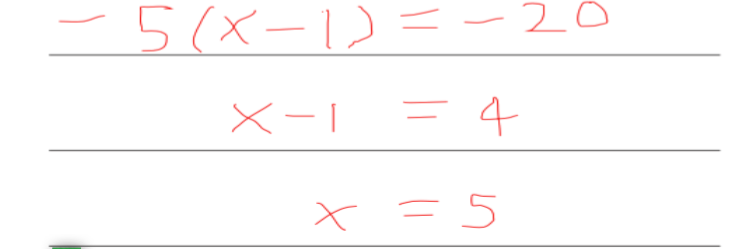
\includegraphics[width=1.1\textwidth,keepaspectratio]{./figure/handwrittenexample.png}
        \caption{Handwritten algebra equations}
        \label{fig:cartpole}
    \end{subfigure}
    %\end{subfigure}
	\begin{subfigure}[l]{0.5\textwidth}
        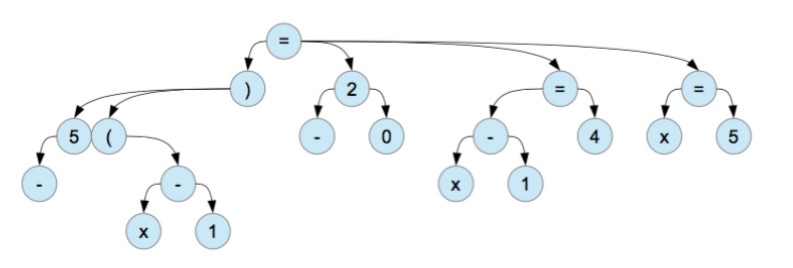
\includegraphics[width=1.1\textwidth,keepaspectratio]{./figure/handwrittentree.png}
        \caption{Dependency tree}
        \label{fig:acrobot}
    \end{subfigure}
    \caption{An example of a set of handwritten algebra equations (a) and its corresponding dependency tree (b).}
    \label{fig:algebra_example}
\end{figure}


Since in the most common dependency parsing setting, there is no immediate reward at every parsing step,
the reward-to-go $Q^e(s,a)$ is computed by using UAS as follows: start from $s$ and apply action $a$, then use expert $\pi^e$ to roll out til the end of the parsing process; $Q^e(s,a)$ is the UAS score of the final configuration. Hence DIL can be considered as directly maximizing the UAS score, while previous approaches such as DAgger or SMILe \cite{Ross2011_AISTATS} tries to mimic expert's actions and hence are not directly optimizing the final objective. 


\end{document} 


